%% Review of Scientific Instruments manuscript — custom induction furnace.
%% Built on REVTeX 4.2 with the AIP substyles (`rsi` journal option) — the class
%% behind the official AIP Publishing template. Template files and the RSI/AIP
%% author guidelines are mirrored in paper/template/rsi/.
%%
%% The earlier HardwareX version of this manuscript (Elsevier elsarticle class)
%% is archived in paper/archive/paper-hardwarex.tex.
%%
%% Build:  make pdf      (pdflatex + bibtex; see paper/Makefile)
%%
\documentclass[%
 aip,
 rsi,%
 amsmath,amssymb,
 reprint,%
]{revtex4-2}

% REVTeX 4.2f (2022) patches LaTeX's tabular internals at \begin{document};
% those patches predate the 2023+ kernel/array rewrite (tagging-ready \@classz
% etc.) and fail with "Extra \or" errors. This manuscript uses standard
% booktabs/tabularx tables (not REVTeX's ruledtabular), so the patching is
% safely disabled.
\makeatletter
\def\switch@tabular{\class@info{REVTeX tabular patching disabled (post-2023 kernel)}}
\let\switch@array\switch@tabular
\makeatother

\usepackage{graphicx}
\usepackage{booktabs}
\usepackage{array}
\usepackage{tabularx}
\usepackage{xcolor}
\usepackage[colorlinks=true,allcolors=blue]{hyperref}
\usepackage{gensymb} % \degree, \celsius
\usepackage[htt]{hyphenat} % allow long \texttt{} paths to break across lines
\sloppy

% Lightweight TODO marker so unresolved items remain visible in the compiled PDF.
\newcommand{\todo}[1]{{\color{red}\textbf{[TODO: #1]}}}

% Convenience column types for wide tables.
\newcolumntype{L}[1]{>{\raggedright\arraybackslash}p{#1}}
\newcolumntype{R}[1]{>{\raggedleft\arraybackslash}p{#1}}

% Validation figures generated by paper/build_validation_figures.py.
\graphicspath{{figures/}}

\begin{document}

\title{Retrofitting a commercial RF induction generator into a
computer-controlled, vacuum-integrated annealing system for reactive-metal
grain growth}

\author{Sterling G. Baird}
\affiliation{Department of Mechanical Engineering, Brigham Young University,
Provo, Utah 84602, USA}
\author{Kevin Cole}
\affiliation{Department of Mechanical Engineering, Brigham Young University,
Provo, Utah 84602, USA}
% \todo{additional authors --- to confirm (add \author/\affiliation pairs here)}

\date{\today}

\begin{abstract}
High-temperature vacuum annealing near a metal's melting point drives controlled
grain growth but normally requires expensive turn-key vacuum induction furnaces.
We describe an open, generator-agnostic modernization stack that converts a bare
commercial RF induction generator into a computer-controlled, vacuum-integrated,
pyrometer-feedback annealing system. The contribution is the reproducible
control/sensing/vacuum layer --- LabVIEW/DAQ analog power control, dual-wavelength
optical temperature feedback, a high-vacuum quartz-tube chamber, and an in-house
machined graphite crucible/susceptor --- which transfers between induction
generators provided the generator exposes a monotonic analog power-control input.
The reproducible build is anchored on the lab's current, USA-sourced generator
(CEIA ``Power Cube'' 6\,kW, procured through East Coast Induction); a $\sim$1970
LEPEL high-frequency furnace served as the originating prototype. We report the
system design, construction and operating procedures, and a performance
validation grounded in $\sim$100 archived anneal logs: a fixed-geometry
power--temperature calibration ($R^2 = 0.991$ over 1200--1400\,\celsius),
repeatable 1200\,\celsius{} / 12\,h Ni4N5 processing ($1201.2 \pm 1.3$\,\celsius{}
across 8 runs), stable long-duration control up to 40\,h at 1325\,\celsius, and
SEM/EBSD/optical microstructural characterization of annealed reactive-metal
specimens cross-referenced to their logged thermal histories. A
tantalum-susceptor/MgO-crucible variant of the same charge stack extends the
furnace to non-coupling ceramics, demonstrated with YSZ. Complete design
files, a costed bill of materials, control software, and the full run-log and
characterization archives are openly available.
\end{abstract}

\keywords{induction furnace; grain growth; vacuum annealing; LabVIEW;
pyrometer; open-source hardware}

\maketitle

\noindent\fbox{\parbox{\linewidth}{\small\textbf{Status:} working draft generated
from the repository's design files, standard operating procedure, parts list,
schematics, and run logs, retargeted from HardwareX to \emph{Review of Scientific
Instruments} (REVTeX 4.2, \texttt{aip,rsi}). \todo{}-marked items flag values or
figures that still need to be confirmed or added before submission; outstanding
bill-of-materials corrections from co-author review are tracked in the pull
request and in Appendix~\ref{app:bom}.}}

%==============================================================
\section{Introduction}
%==============================================================

High-temperature annealing near a metal's melting point drives controlled
\textbf{grain growth}, which is central to studying microstructure--property
relationships in metals such as nickel and
iron~\cite{liu2021studyofgrain,mohrbacher2026applicationofmicroalloying,alogab2007theinfluenceof}.
Doing this without oxidizing the sample requires both high temperature
($\sim$1400--1500\,\celsius) and high vacuum (or inert
atmosphere)~\cite{zhornyak1982reductionanddecarburization,muramatsu2005gascontaminationdue}.
Commercial vacuum induction annealing furnaces that meet these requirements are
expensive turn-key systems, which puts them out of reach for many academic labs.

This work takes the opposite approach: rather than building or buying a complete
furnace, we \textbf{retrofit and modernize a bare RF induction generator} into a
full annealing system by adding (1)~computer power control, (2)~closed-loop optical
temperature control, (3)~a high-vacuum quartz-tube chamber, and (4)~a machined
graphite crucible/susceptor. The emphasis of the contribution is the
\textbf{modernization stack itself}, which is deliberately
\textbf{generator-agnostic}: the same control software, vacuum chamber, pyrometer
feedback, crucible, and work-coil geometry transfer from one induction generator to
another. The only requirement a reader's generator must satisfy is an \textbf{analog
power-control input with a monotonic command$\rightarrow$power response} over the
usable range (e.g. 4--20\,mA, 0--5\,V, or 0--5\,mA); near-linearity is convenient but
not required, because the pyrometer feedback and PID calibration absorb any
nonlinearity. That portability is the reproducible result and is what makes the
design reusable by other labs that already own, or can buy, such an induction
generator.

A second feature that broadens the system's applicability is the \textbf{machined
graphite crucible/susceptor}: because graphite couples strongly to the RF field and
heats the charge indirectly by conduction and radiation, the furnace is not limited
to electrically conductive samples --- it can also process poorly- or non-coupling
materials such as YSZ ceramic. This makes the same build useful well beyond
reactive-metal annealing.

The modernization was first prototyped on a $\sim$1970 LEPEL high-frequency
induction furnace owned by the BYU Mechanical Engineering department --- at the time
the only departmental machine able to reach the Ni/Fe melting range. A ``remote
control'' capability was added in August 2019 to drive the generator's power from a
computer instead of the front-panel knob. The lab subsequently moved the same stack
onto a current, USA-sourced solid-state generator (CEIA ``Power Cube'' 6\,kW via
East Coast Induction), whose Power Controller C-V3 Plus accepts a standard analog
(4--20\,mA) power setpoint. An intermediate, separately-purchased import generator
(CYSI GP-15A) was evaluated but did not meet the lab's control requirements --- the
required analog remote-control input was lost across vendor model substitutions ---
and was retired. The reproducible build documented here therefore targets the
current USA generator, with the LEPEL retrofit retained as historical context.

Compared with commercial vacuum annealing furnaces, this approach has
\textbf{substantially lower capital cost} (the generator + heating head +
controller + chiller package was quoted at $\approx$\$16.5k in 2021, and the
retrofit components are itemized in Appendix~\ref{app:bom}, versus
\$50k--\$200k+ for turn-key systems), is repairable and modifiable by the user,
and is broadly reusable: any lab with an induction generator and an analog power
input can reproduce the control, vacuum, and temperature-sensing additions
described below. The system is aimed at:

\begin{itemize}
\item materials labs needing \textbf{oxidation-free grain-growth anneals} of
reactive metals (Ni, Fe) near their melting points;
\item labs that own a \textbf{bare induction generator} and want to add computer
setpoint control, optical feedback, and vacuum integration without buying a
turn-key furnace;
\item groups processing \textbf{poorly- or non-coupling charges} (e.g. YSZ
ceramic) that can be heated indirectly through the graphite susceptor; and
\item teaching/maker contexts wanting a \textbf{repairable, modifiable}
high-temperature vacuum furnace built from documented, open design files.
\end{itemize}

All design files, control software, run logs, and characterization data are
openly available: the development repository is
\url{https://github.com/vertical-cloud-lab/custom-induction-furnace} and an
archival snapshot is deposited at Zenodo
(\href{https://doi.org/10.5281/zenodo.20878017}{10.5281/zenodo.20878017}), with
hardware design files under the CERN-OHL-S v2 license and control code under the
MIT license (proposed).

\subsection{Scope and reproducibility boundary}

To be explicit about what this paper does and does not reproduce: \textbf{this work
does not reproduce the RF generator internals.} It reproduces the \emph{modernization
layer} built around a compatible generator --- the computer power control, optical
(pyrometer) feedback, high-vacuum quartz-tube chamber, machined graphite
crucible/susceptor, work-coil geometry, and the mechanical support fixturing. A
reader supplies (or already owns) a compatible generator and rebuilds the layer
described here.

\subsection{Prior art and comparison}

Three classes of alternative exist, and each presents a limitation this design
addresses. Commercial vacuum induction annealing furnaces are turn-key systems
costing \$50k--\$200k+; they are closed, difficult to modify or repair in-house,
and carry vendor lock-in. Openly documented resistively heated tube and box
furnaces reach lower maximum temperatures with slower ramps than induction
heating, and offer no RF-susceptor route to heating a non-coupling charge.
Finally, induction generators themselves are widely available as bare industrial
units (CEIA, Ambrell, and others), but ship without integrated vacuum, optical
temperature feedback, or computer setpoint control --- exactly the layer this
work adds.

%==============================================================
\section{System design and description}
%==============================================================

\subsection{Architecture and control signal flow}

The system comprises five subsystems, shown in the labeled overview schematic of
Fig.~\ref{fig:overview} (the editable source schematics are in
\texttt{docs/induction-furnace-schematic.pptx} and are extracted to text in
\texttt{paper/extracted-context/}); Fig.~\ref{fig:furnacephoto} shows the
corresponding assembled system at operating power:

\begin{figure}[ht]
\centering
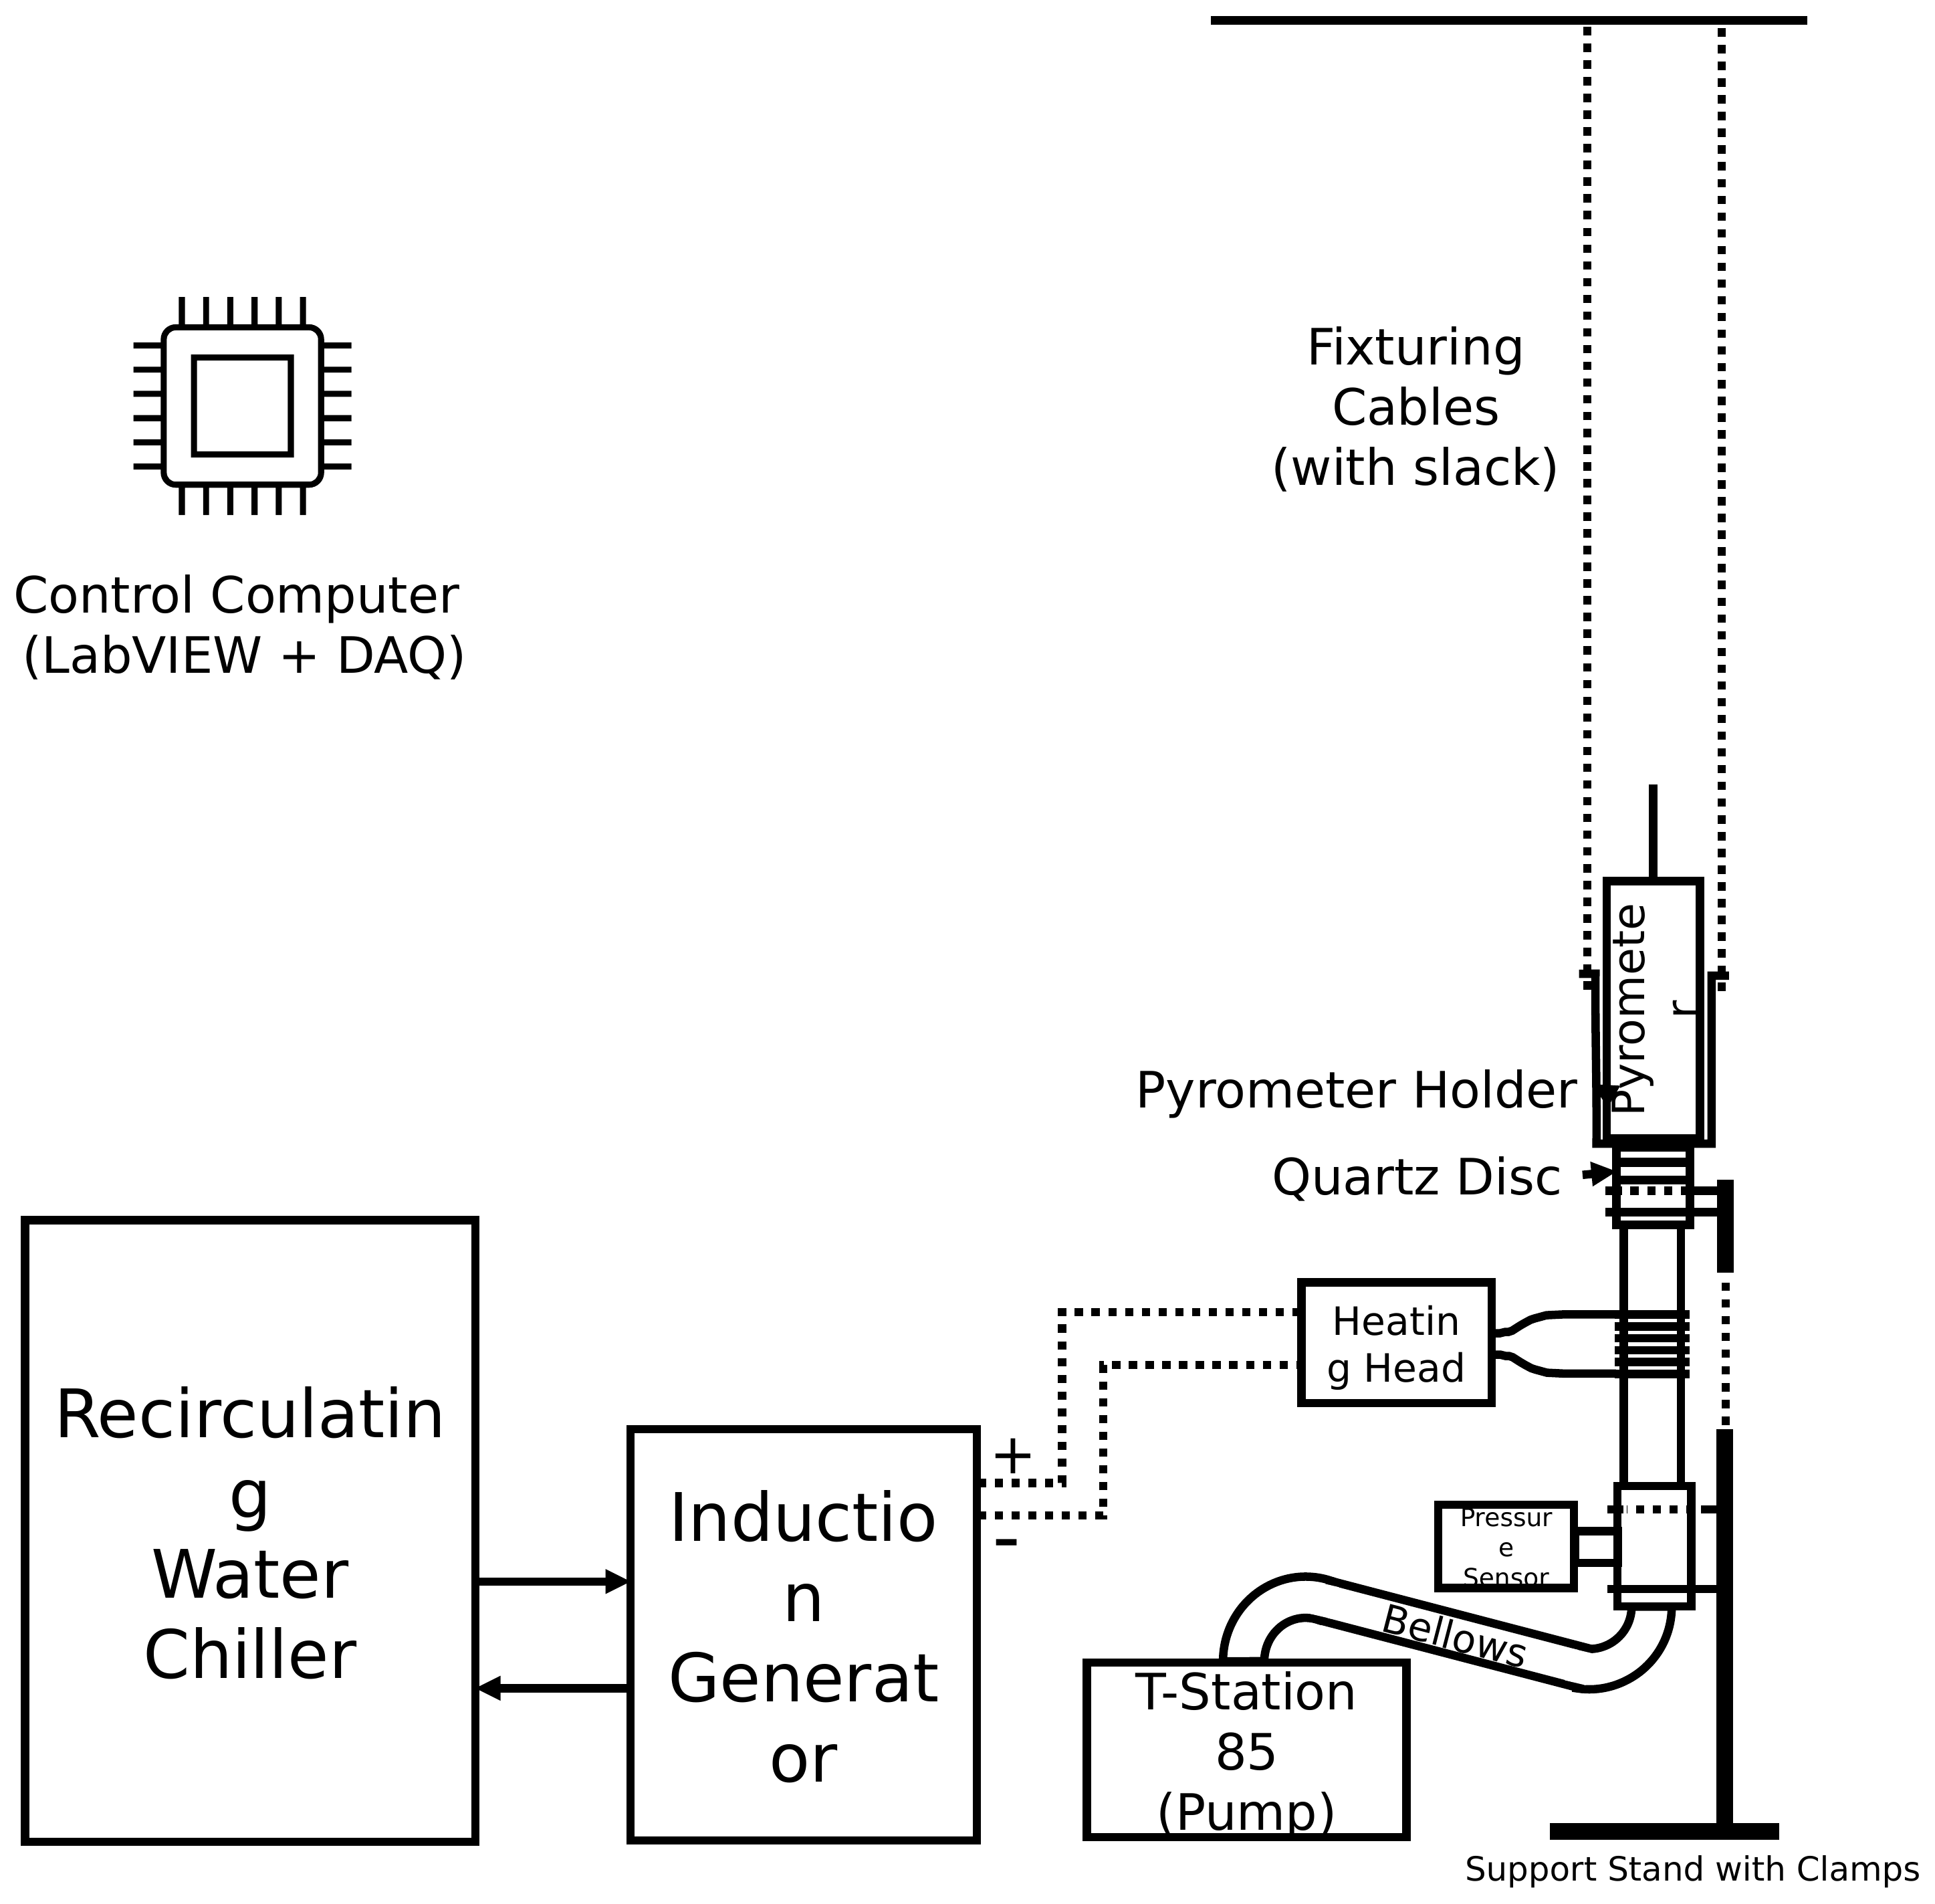
\includegraphics[width=\linewidth]{fig_system_overview.png}
\caption{System overview of the computer-controlled, vacuum-integrated induction
annealing system: recirculating water chiller and induction generator drive a
water-cooled heating head/work coil around a quartz-tube vacuum chamber; a
dual-wavelength pyrometer sights the charge through a quartz optical disc; an Edwards
T-Station~85 turbo-molecular pump (with pressure gauge and bellows) evacuates the
chamber; and a DAQ/laptop sets generator power and reads the pyrometer for
closed-loop control. Rendered from the editable source schematic
\texttt{docs/induction-furnace-schematic.pptx}.}
\label{fig:overview}
\end{figure}

\begin{enumerate}
\item \textbf{RF generator + work coil.} A solid-state induction generator (current
build: CEIA Power Cube PW3-90/50) drives a water-cooled copper work coil. The coil
carries both the oscillating current and cooling water. Coil geometry ($\sim$3\,in
tall, 2.5\,in ID, $\sim$6.5 turns) was tuned to the sample/crucible
stack~\cite{vankan2024electromagneticinductionheating} (see
\texttt{extracted-context/order\_corrections\_coils.md}).

\item \textbf{Vacuum + gas.} A quartz tube forms the chamber and is connected through
a KF40 flange and flexible bellows to an Edwards T-Station 85 turbo-molecular pump
($\sim$1$\times$10$^{-6}$--10$^{-8}$\,Torr). A manual vent valve and an inert-gas
regulator allow controlled venting/backfilling to suppress oxidation of reactive
metals. The vacuum connection stack, in order, is: \textbf{quartz tube $\rightarrow$
KF40 flange + optical window $\rightarrow$ flexible bellows $\rightarrow$ vacuum
gauge $\rightarrow$ Edwards T-Station 85 $\rightarrow$ vent / inert-gas backfill
branch.}

\item \textbf{Optical temperature sensing.} A dual-wavelength (ratio) pyrometer (the
canonical unit is a LumaSense IMPAC ISR 6, 800--2500\,\celsius; the IMPAC brand is
LumaSense's) views the sample through a KF40 optical window, providing a non-contact
temperature signal that is robust to emissivity changes and to the RF field that
would corrupt thermocouples~\cite{ham2016insituspectralemissivity,suleiman2025improvingpyrometryof,usamentiaga2014infraredthermographyfor}.

\item \textbf{Control / DAQ + LabVIEW.} A LabVIEW DAQ analog output sets generator
power; the pyrometer signal is read back for closed-loop ramp/soak control. The VIs
implement manual control, automated ramping, PID tuning, and email alerts (see
\texttt{code/} in the repository). In the CEIA build the DAQ outputs \textbf{0--5\,V}
to a \textbf{voltage-to-current loop conditioner} that converts the command to the
controller's \textbf{4--20\,mA} power-setpoint input (the LEPEL prototype instead
took a 0--5\,mA command directly). The closed-loop \textbf{signal flow} is therefore:
\textbf{LabVIEW setpoint $\rightarrow$ DAQ analog output (0--5\,V) $\rightarrow$
V$\rightarrow$I conditioner (4--20\,mA) $\rightarrow$ generator power $\rightarrow$
sample/crucible heating $\rightarrow$ pyrometer optical reading $\rightarrow$ DAQ
analog input (scaled to \celsius) $\rightarrow$ PID controller $\rightarrow$ updated
analog command.} The same path runs \textbf{open-loop} (direct command ramp) while
the temperature is below the pyrometer's $\sim$700\,\celsius{} detection floor; once
the pyrometer reports a \textbf{sustained valid reading above that floor}, control
hands over to \textbf{closed-loop} PID on the optical temperature~\cite{meng2023designofvacuum}.

\item \textbf{Mechanical support stand + crucible.} A bolted support stand (8 short +
4 long sections, 12 corner braces, 4 floor mounts) positions the chamber, coil,
pyrometer holder, and quartz disc. An \textbf{in-house machined graphite crucible}
holds the sample and acts as the RF susceptor.
\end{enumerate}

The LabVIEW control front panel (Fig.~\ref{fig:controlpanel}) exposes the ramp-up,
PID-soak, and cool-down setpoint tables, the PID gains, the inert-gas flow control,
and live power-command and pyrometer-temperature traces used to run and monitor an
anneal.

\begin{figure}[ht]
\centering
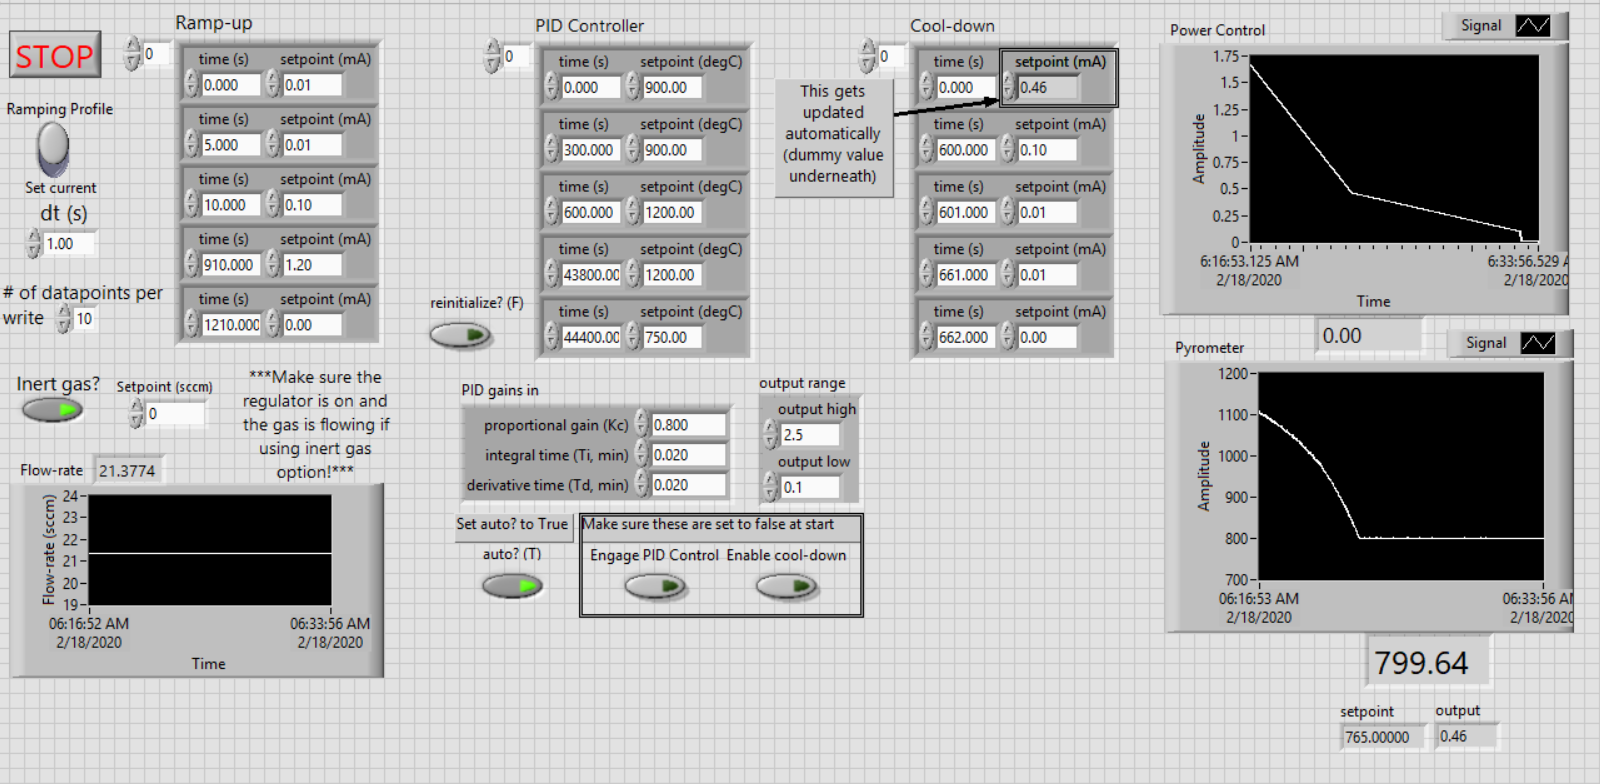
\includegraphics[width=\linewidth]{fig_control_panel.png}
\caption{LabVIEW control front panel (\texttt{docs/equipment-reference/frontPanel\_200219.PNG}):
editable ramp-up / PID-soak / cool-down setpoint tables (time vs.\ analog command in
mA below the pyrometer floor and vs.\ \celsius{} once closed-loop), PID gains and
output range, inert-gas flow setpoint/readback, and live power-command and
pyrometer-temperature strip charts. Here the pyrometer reads $\sim$800\,\celsius{}
during ramp.}
\label{fig:controlpanel}
\end{figure}

\subsection{Technical specifications}

Table~\ref{tab:techspecs} lists the technical specifications of the build documented
here. These are \emph{build-dependent} values: a reader supplies their own generator,
pump, and pyrometer and re-establishes the corresponding values for their build.

\begin{table*}[ht]
\caption{Technical specifications of the documented build. These are
build-dependent values that a reader replaces with their own
generator/pump/pyrometer equivalents.
\label{tab:techspecs}}
\small
\begin{tabularx}{\linewidth}{>{\raggedright\arraybackslash}p{0.30\linewidth} X}
\toprule
\textbf{Specification} & \textbf{Value (this build)} \\
\midrule
Induction generator (reproducible build) & CEIA ``Power Cube'' PW3-90/50 solid-state RF generator + Power Controller C-V3 Plus (East Coast Induction, USA) \\
Induction generator (prototype) & LEPEL high-frequency tube furnace ($\sim$1970), up to $\sim$35\,kW \\
Power-control input & 4--20\,mA analog setpoint via LabVIEW/DAQ $\rightarrow$ V$\rightarrow$I conditioner (CEIA build; the LEPEL prototype used 0--5\,mA) \\
Max sample temperature & $\sim$1400--1500\,\celsius+ (Ni/Fe melting range); $\sim$1700\,\celsius{} with the tantalum/MgO ceramic stack (Sec.~\ref{sec:ysz}) \\
Pyrometer detection range & $\sim$800--2500\,\celsius{} (dual-wavelength ratio); does not report below $\sim$700\,\celsius \\
Demonstrated soak duration & minutes up to $\sim$40\,h (per \texttt{docs/data\_log/} run logs) \\
Sample / crucible envelope & charge fits inside a 35\,mm-ID quartz tube and a machined graphite crucible \\
Operating vacuum & $\sim$1$\times$10$^{-6}$ to 1$\times$10$^{-8}$\,Torr (turbo-molecular pump) \\
Temperature measurement & Dual-wavelength ratio pyrometer (LumaSense IMPAC ISR 6, $\sim$800--2500\,\celsius) \\
Chamber & Quartz tube, KF40 optical-window flange, inert-gas vent \\
Crucible / susceptor & In-house machined graphite (3000\,\celsius{} grade) crucible-susceptor \\
Work coil & Water-cooled copper, $\sim$3\,in tall, 2.5\,in ID, $\sim$6.5 turns \\
\bottomrule
\end{tabularx}
\end{table*}

\subsection{Generator compatibility and portability}
\label{sec:portability}

The control/sensing/vacuum layer transfers to any generator that meets these
criteria:

\begin{itemize}
\item Exposes an \textbf{external analog power-control input} (e.g. 4--20\,mA or 0--5\,V/0--5\,mA).
\item The command$\rightarrow$delivered-power response is \textbf{monotonic over the usable range} (near-linear is convenient but not required, since the pyrometer feedback closes the loop).
\item Supports a \textbf{water-cooled induction head/coil} matching the documented coil dimensions.
\item Delivers \textbf{enough RF power} to reach the target temperature for the documented crucible/sample stack.
\item Allows \textbf{safe electrical isolation} between the DAQ/control path and the generator input.
\item Has the required cooling and line power for the selected generator.
\end{itemize}

When porting to a new generator, the following must be re-established:
analog-command scaling, power-to-temperature calibration, PID gains, coil/sample
alignment, maximum safe ramp rate, and any generator-specific interlock behavior.
The port from the $\sim$1970 LEPEL prototype to the current CEIA build is the
existence proof for this portability claim: the dual-wavelength pyrometer
feedback, the quartz-tube/KF40 vacuum chamber, the machined graphite
crucible/susceptor, the bolted support stand, and the LabVIEW/DAQ control VIs
all transferred unchanged. Only the analog interface itself differed --- the
LEPEL took a 0--5\,mA command directly, whereas the CEIA Power Controller C-V3
Plus expects 4--20\,mA, hence the V$\rightarrow$I loop conditioner --- and the
power--temperature calibration and PID gains were re-established for the new
generator, as they must be for any port. The generator's internal operating
frequency ($\sim$200--450\,kHz vacuum-tube LEPEL vs.\ the solid-state CEIA's
self-set frequency) and maximum power ($\sim$35\,kW vs.\ 6\,kW) sit behind the
analog interface and required no change to the stack beyond re-tuning power for
the charge.

\subsection{Custom-machined graphite crucible / susceptor}

Because some charges of interest couple poorly to the RF field (e.g. YSZ ceramic) or
must be physically contained, the sample is held in a \textbf{graphite crucible
machined in-house from 3000\,\celsius-grade graphite stock} (Cotronics 56L-3). The
graphite couples strongly to the induction field and acts as a \textbf{susceptor},
transferring heat to the contained charge by conduction/radiation; this makes the
same furnace usable for conductive metals (direct coupling) and for non/poorly-coupling
materials (indirect, susceptor-driven heating). Crucibles are machined to fit inside
the quartz tube and seat on a ceramic-cylinder / Teflon spacer stack. Cracked
crucibles are repaired with a 3000\,\celsius{} graphite cement (Resbond 931) rather
than discarded. The two-piece geometry --- a cup body and a lidded cap with a
central bore --- contains the charge while leaving an optical path for the
pyrometer to sight the sample (Fig.~\ref{fig:crucible}). The measured dimensions
of every piece in the stack (crucible body, lid, alumina spacer discs, and
sapphire pyrometer window) are given in Fig.~\ref{fig:crucible-dims}; fully
assembled, the crucible stack stands 13\,mm tall. The
specimen-loading sequence --- specimen sandwiched between two alumina sheets in
the cup body, lid seated on top, and sapphire window placed over the lid bore
--- is shown step by step in Fig.~\ref{fig:crucible-assembly}. For ceramic
charges requiring soak temperatures beyond the graphite/alumina stack's service
range, the crucible stack is exchanged for a tantalum-susceptor/MgO-crucible
variant described in Sec.~\ref{sec:ysz}.

\begin{figure}[ht]
\centering
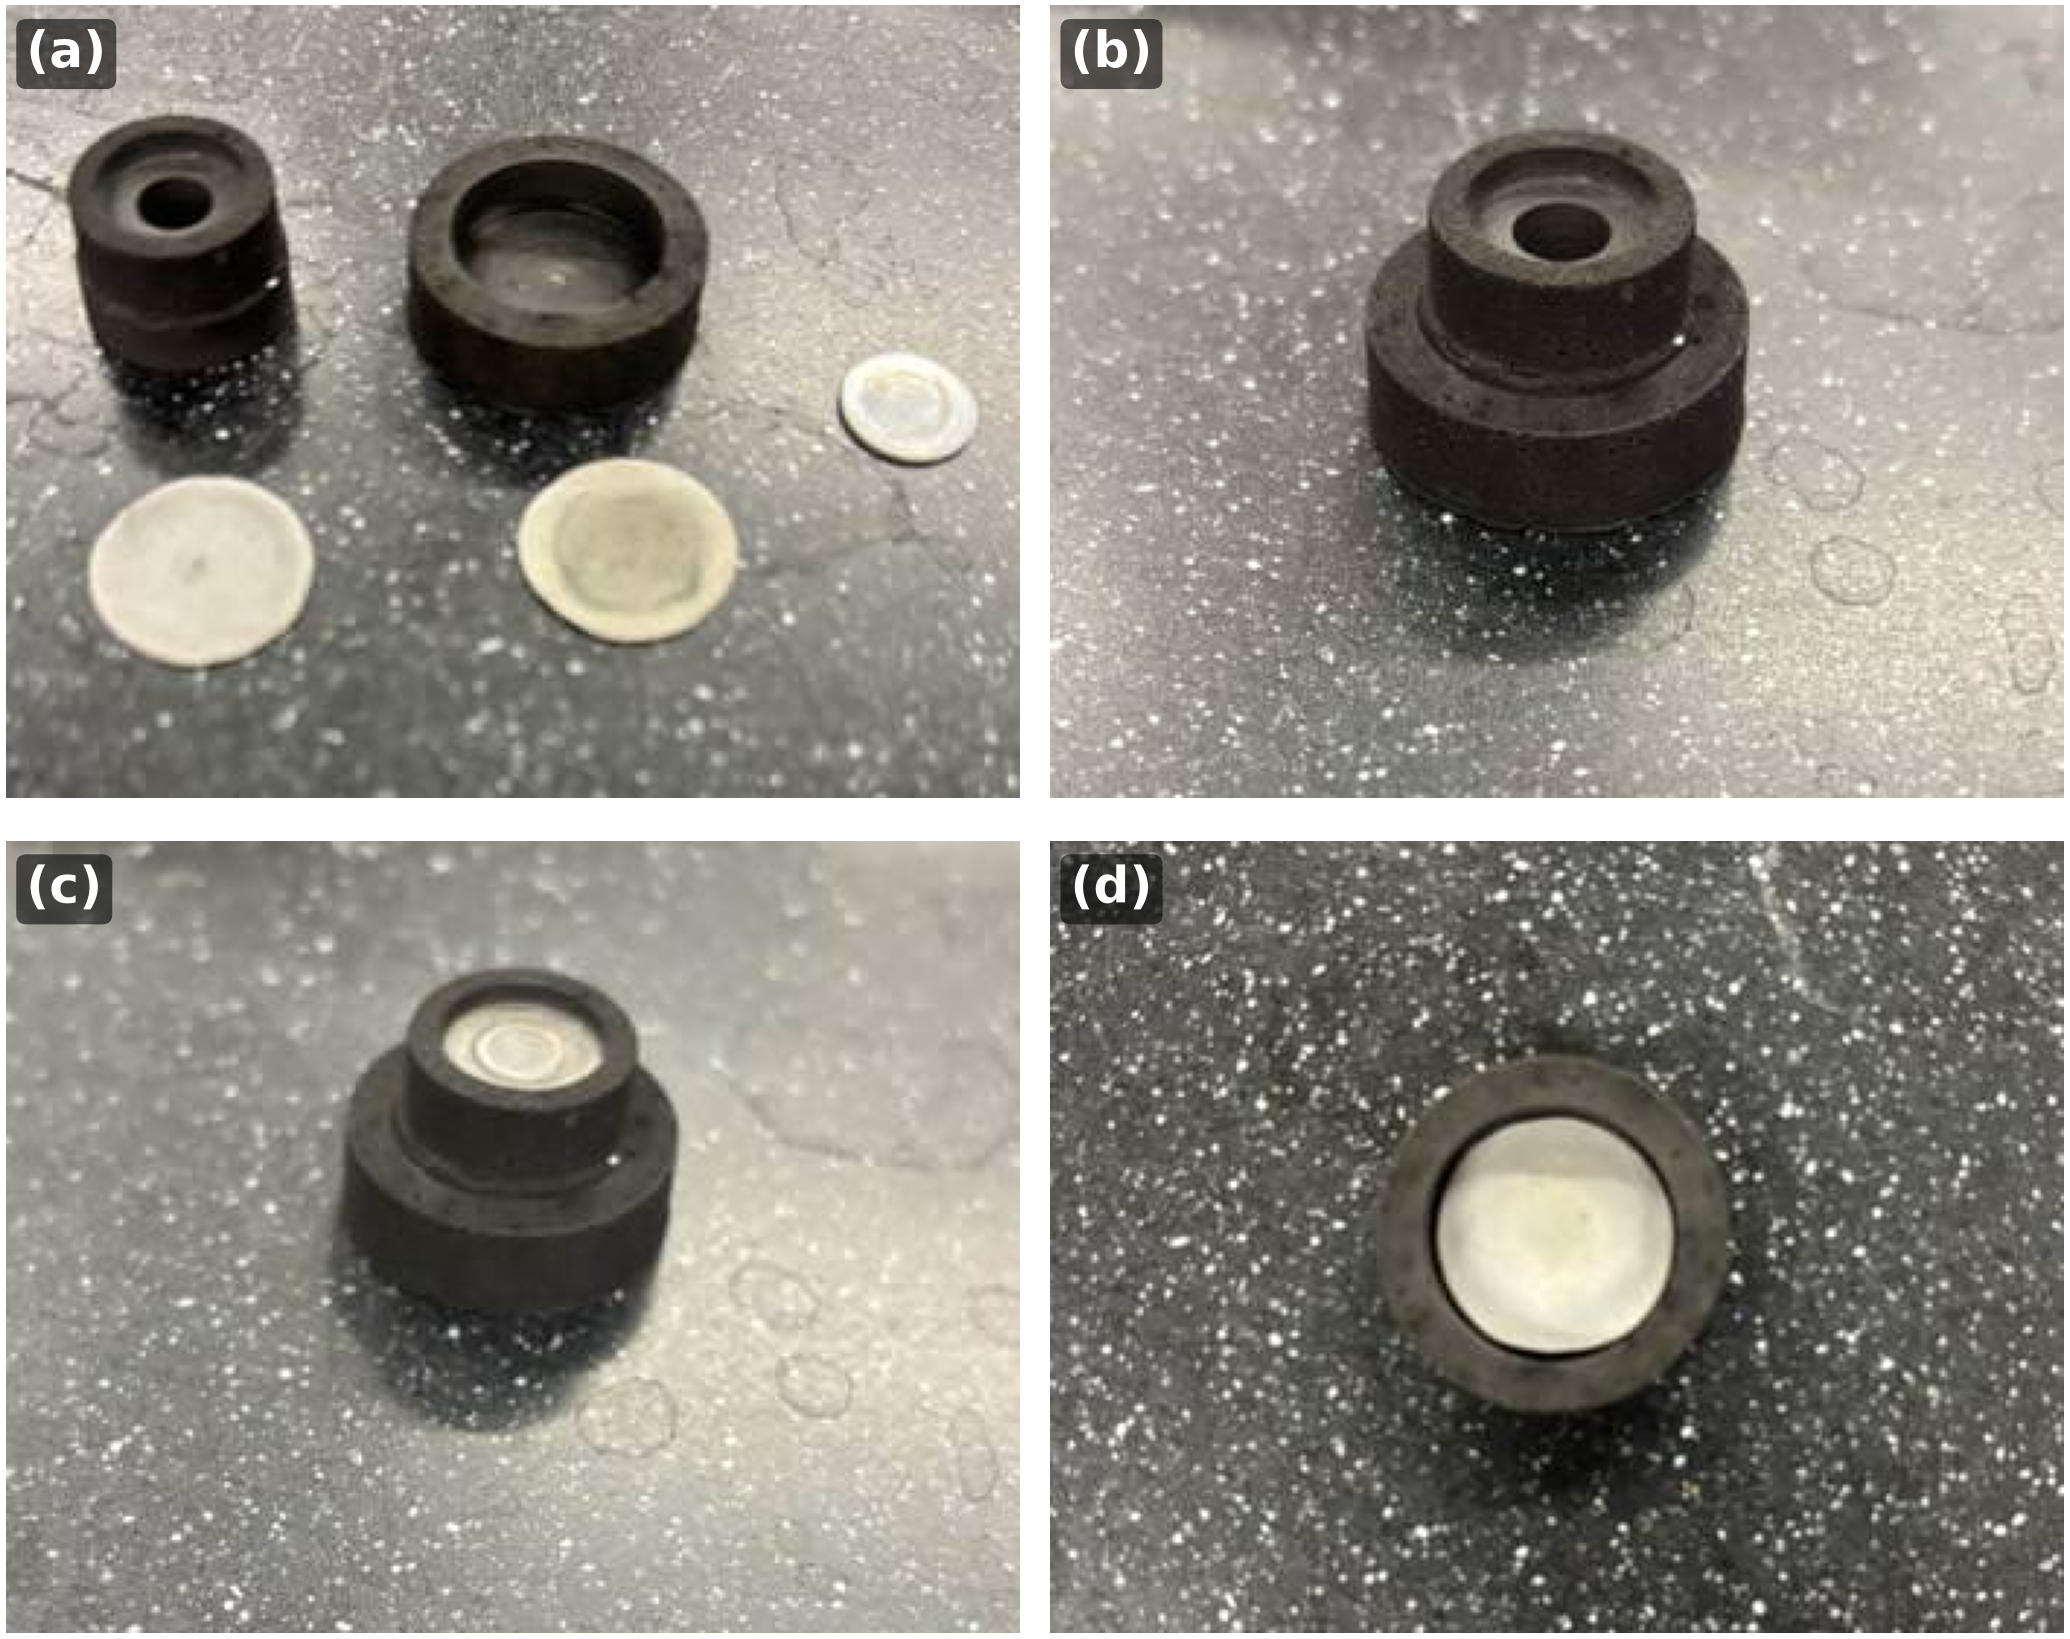
\includegraphics[width=0.75\linewidth]{fig_crucible.png}
\caption{Fully disassembled graphite crucible. Top left is the crucible lid, top
middle is the bottom of the crucible that acts as the specimen carrier, far right
is the sapphire window, bottom left and middle are the alumina
sample-surrounding sheets.
\label{fig:crucible}}
\end{figure}

\begin{figure}[ht]
\centering
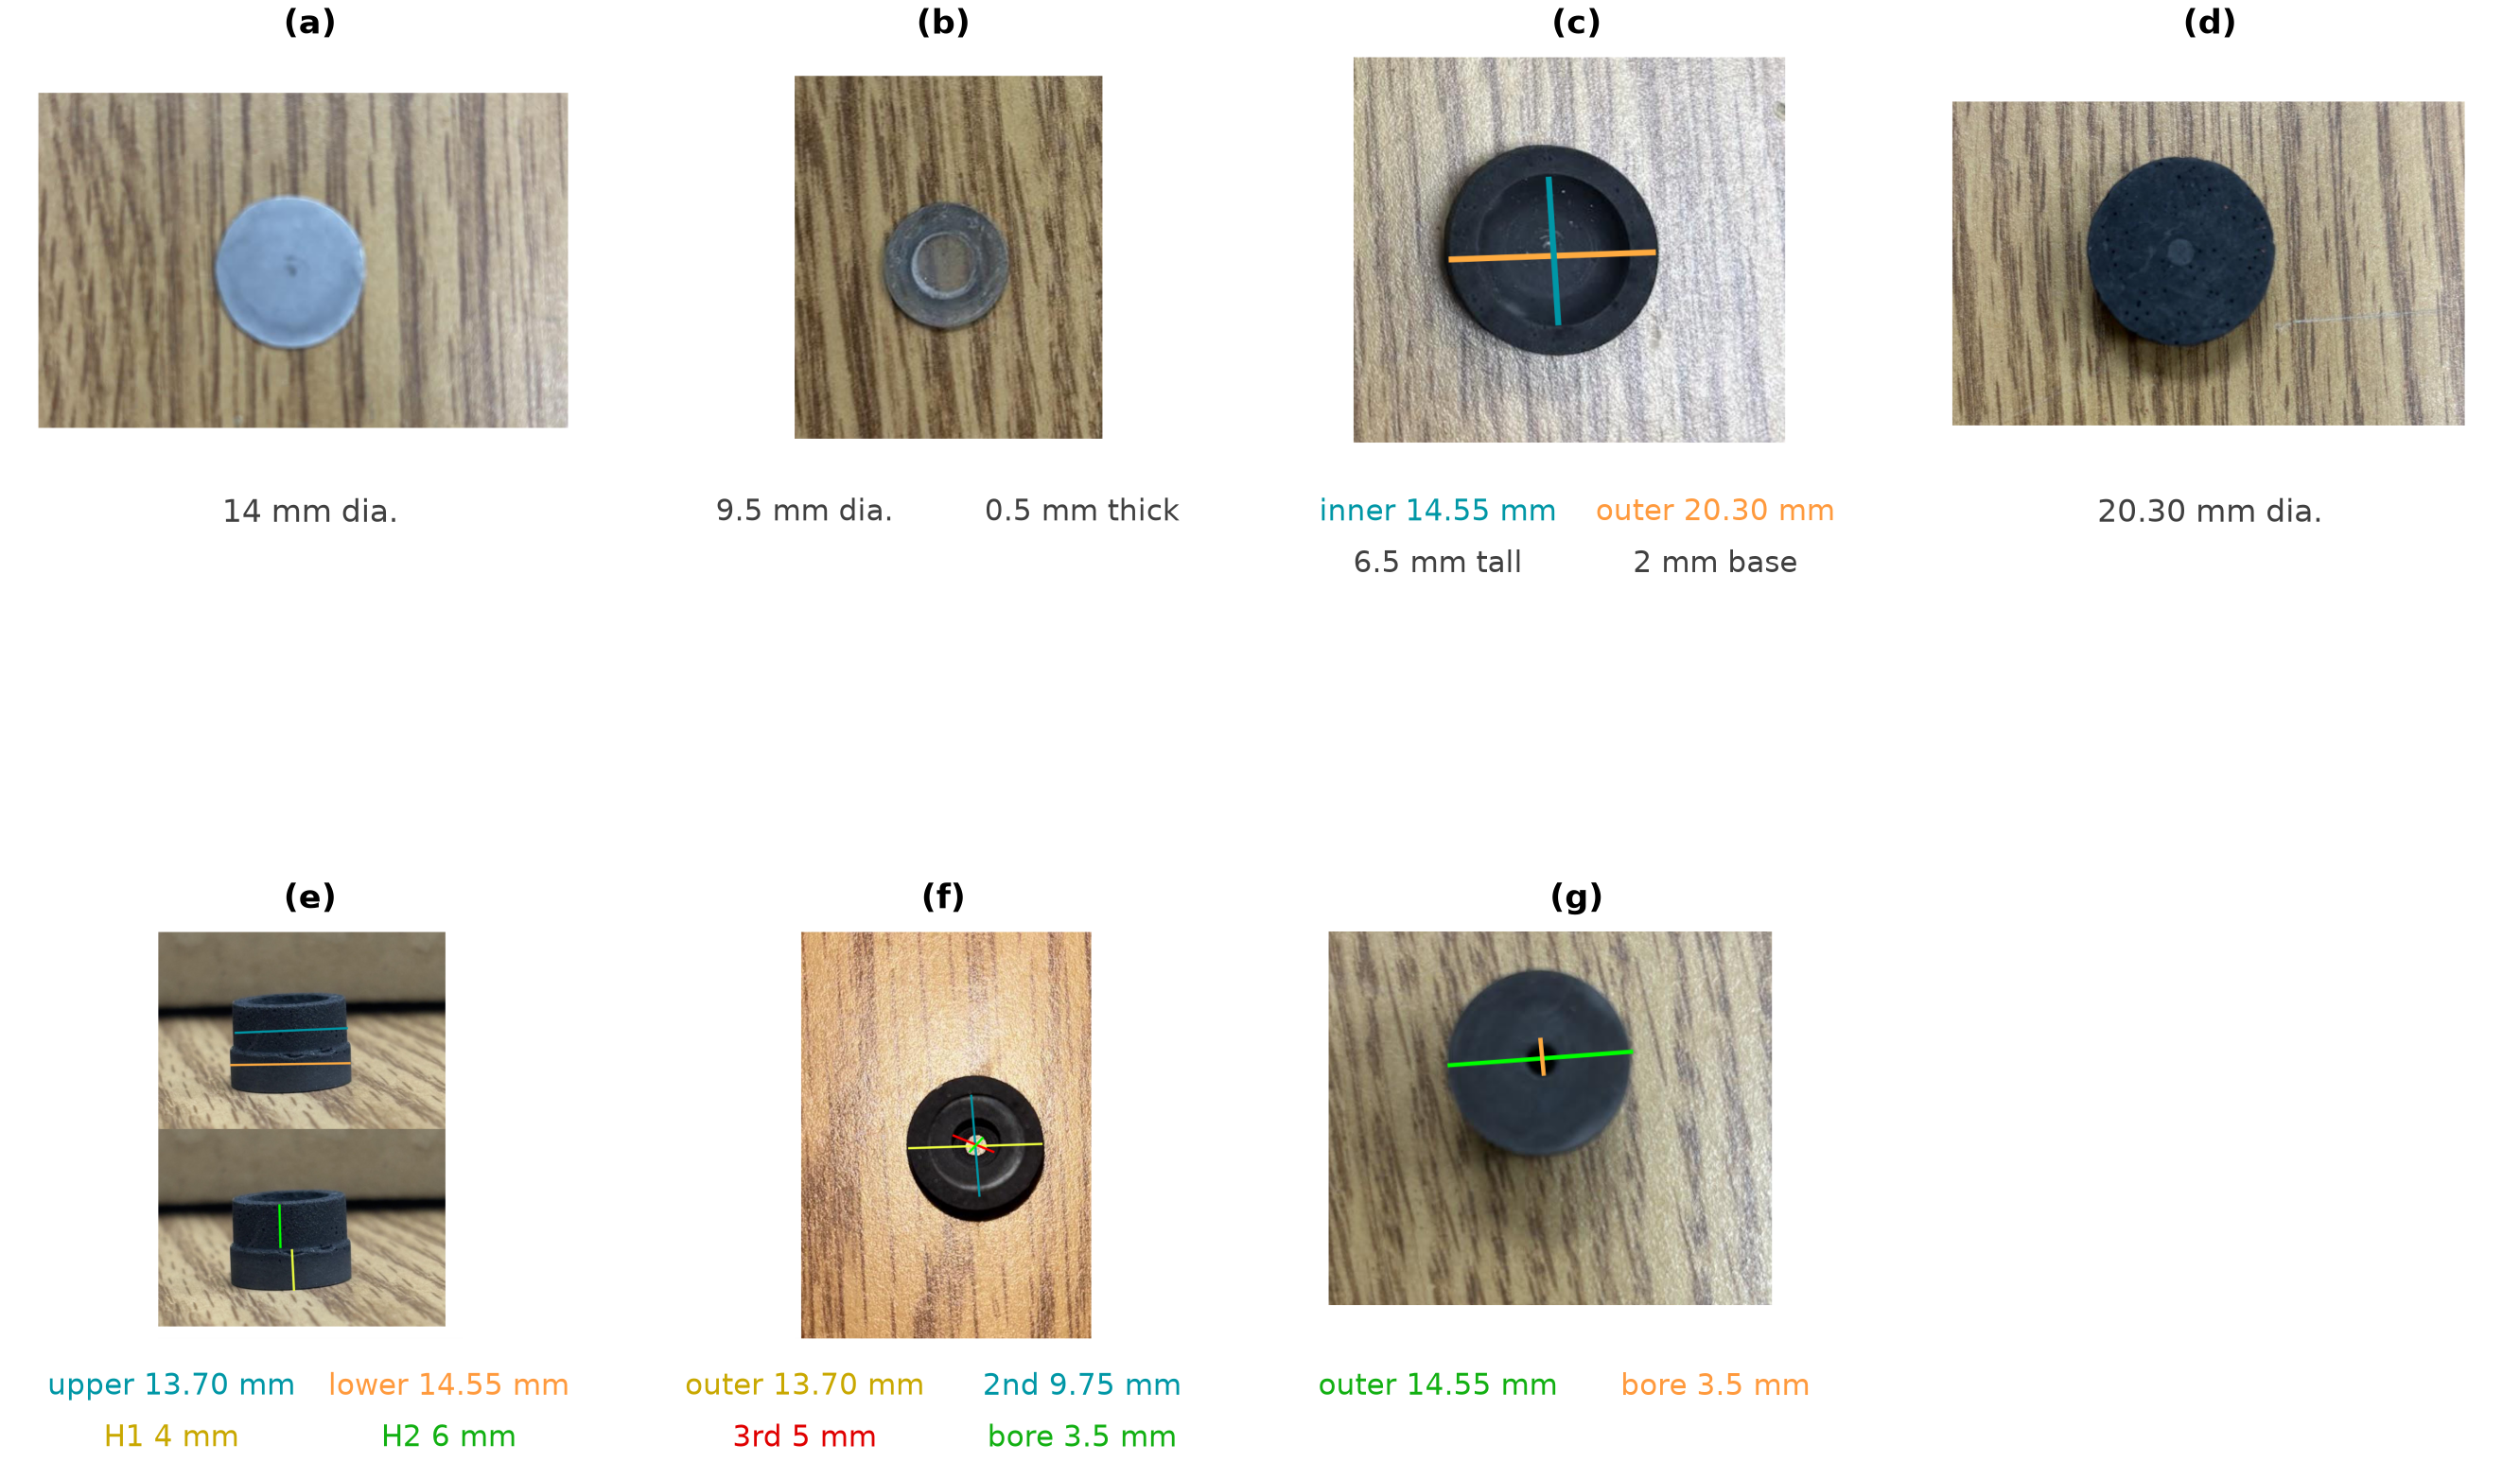
\includegraphics[width=\linewidth]{fig_crucible_dimensions.png}
\caption{Measured dimensions of each part of the graphite crucible/susceptor
stack, with the coloured measurement lines drawn on the corresponding
photograph. (a)~Alumina spacer disc, 14\,mm dia. (b)~Sapphire pyrometer window,
9.5\,mm dia., 0.5\,mm thick. (c)~Crucible body, top: machined sample cavity
14.55\,mm ID (teal), 20.30\,mm OD (orange); the cup is 6.5\,mm tall with a 2\,mm
base. (d)~Crucible body, bottom face, 20.30\,mm dia. (e)~Crucible lid, oblique:
the stepped plug seats into the cavity --- 13.70\,mm upper step (teal),
14.55\,mm lower shoulder (orange); the upper step is 4\,mm tall (H1, yellow) and
the lower shoulder 6\,mm tall (H2, green). (f)~Crucible lid, top: four concentric
steps of 13.70\,mm (outermost), 9.75\,mm, 5\,mm, and a 3.5\,mm central
pyrometer-sighting bore. (g)~Crucible lid, bottom: 14.55\,mm seating face (green)
and the 3.5\,mm through-bore (orange). Two alumina discs sandwich the specimen
inside the cavity, the lid seats on top, and the sapphire window closes the bore
so the pyrometer sights the sample through the lid; fully assembled the stack
stands 13\,mm tall. Measurements contributed by R.~Guymon.
\label{fig:crucible-dims}}
\end{figure}

\begin{figure}[ht]
\centering
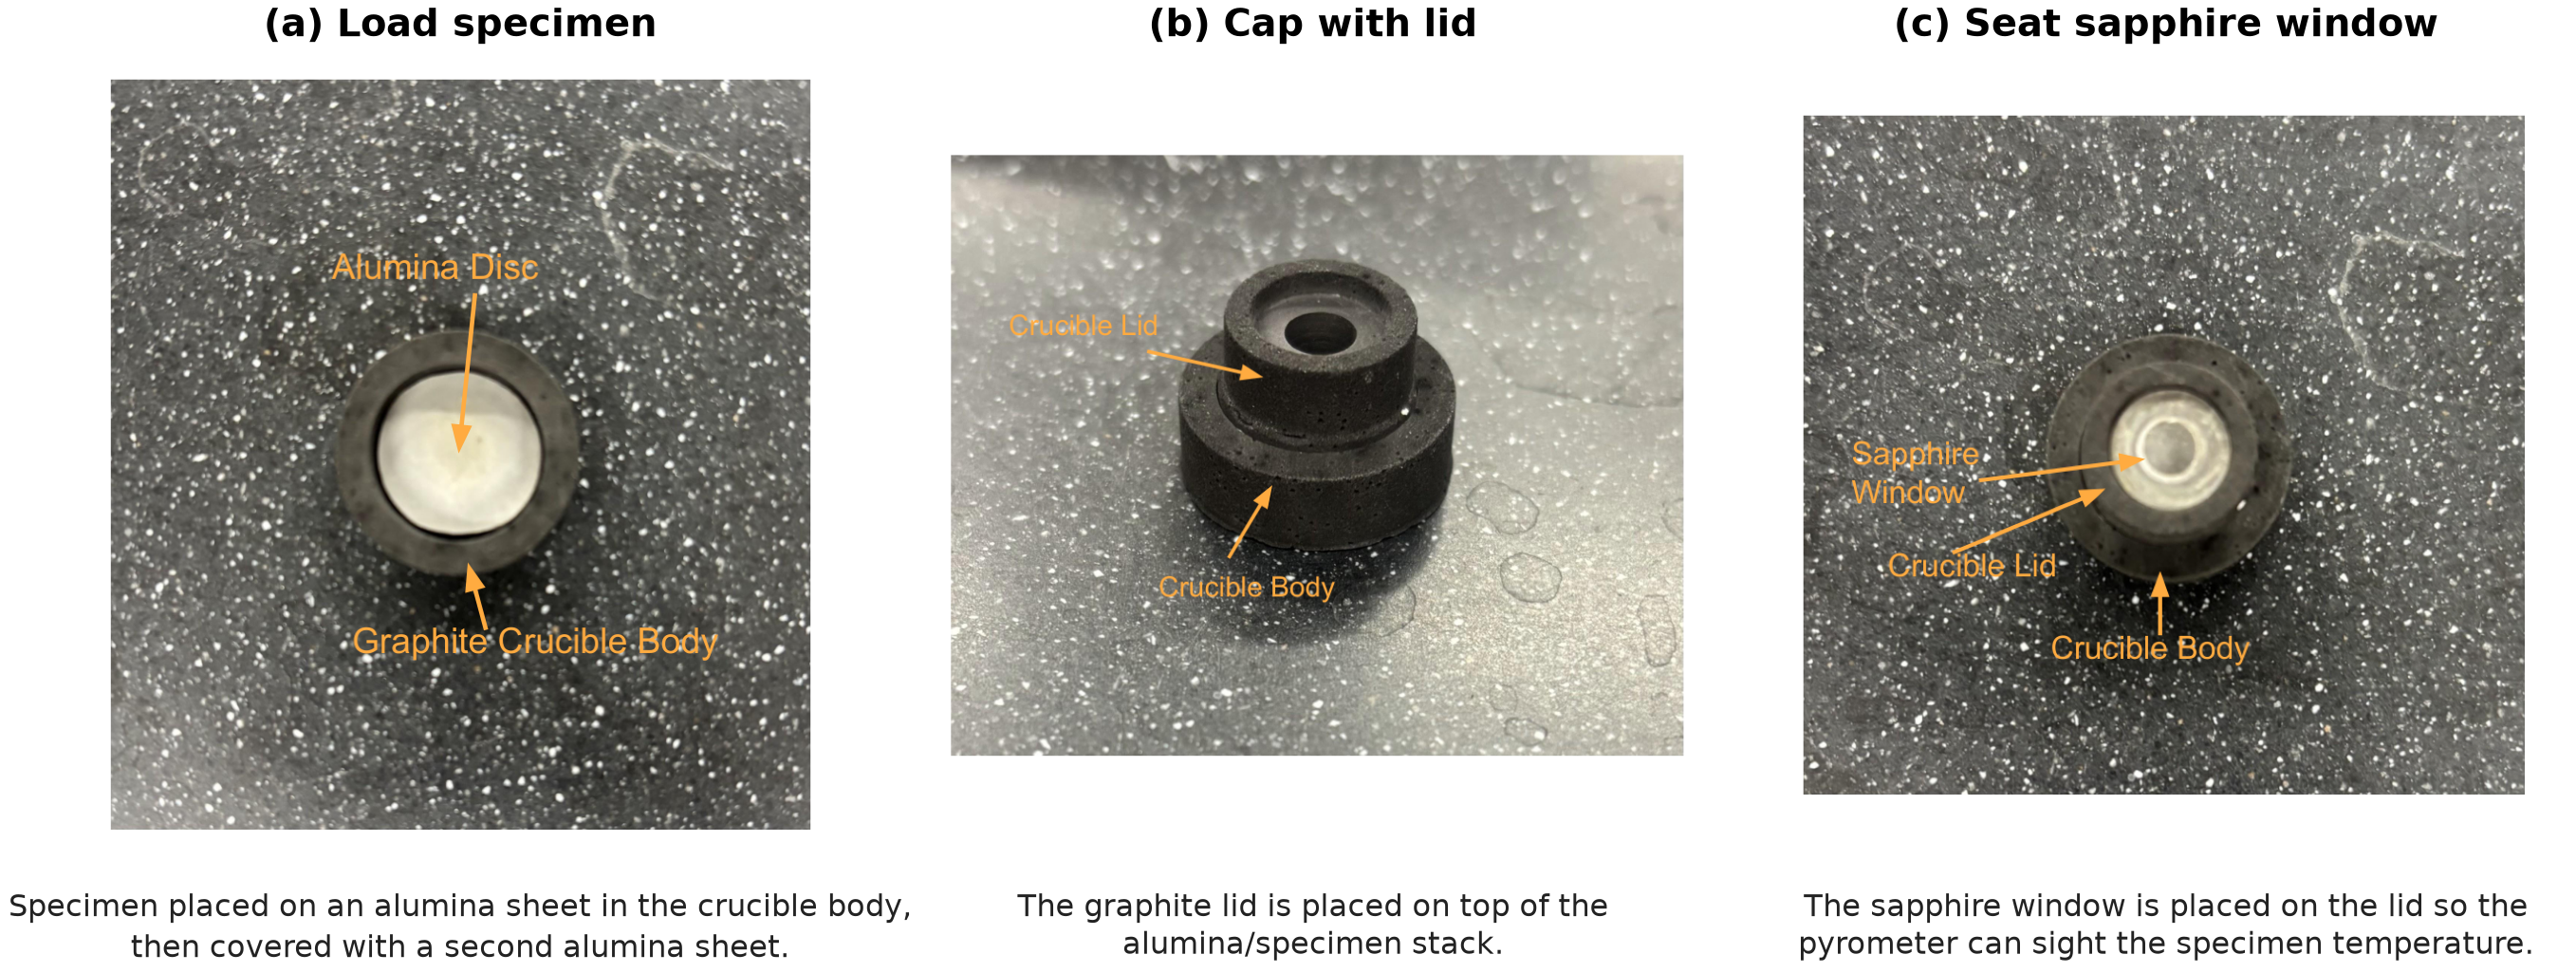
\includegraphics[width=\linewidth]{fig_crucible_assembly.png}
\caption{Specimen-loading sequence for the graphite crucible/susceptor, in order
(orange call-outs name the visible parts). (a)~The specimen is placed on an
alumina sheet in the crucible body and covered with a second alumina sheet, so
the alumina discs isolate the specimen from the graphite. (b)~The graphite lid is
seated on top of the alumina/specimen stack. (c)~The sapphire window is placed
over the lid bore, closing the crucible while leaving an optical path for the
pyrometer to sight the specimen temperature through the window.
Photographs contributed by R.~Guymon.
\label{fig:crucible-assembly}}
\end{figure}

%==============================================================
\section{Construction and operation}
%==============================================================

\subsection{System assembly}

This section describes how the subsystems of Fig.~\ref{fig:overview} are
physically connected, following the heating, vacuum, gas, and control paths in
turn; the costed part list is in Appendix~\ref{app:bom} and the design files
(coil drawing, editable schematics, STEP models) in
Appendix~\ref{app:designfiles}. Figure~\ref{fig:furnacephoto} shows the
assembled system at operating power, and Fig.~\ref{fig:vacuumdetails} details
the vacuum and gas-handling connections described below.

\begin{figure}[ht]
\centering
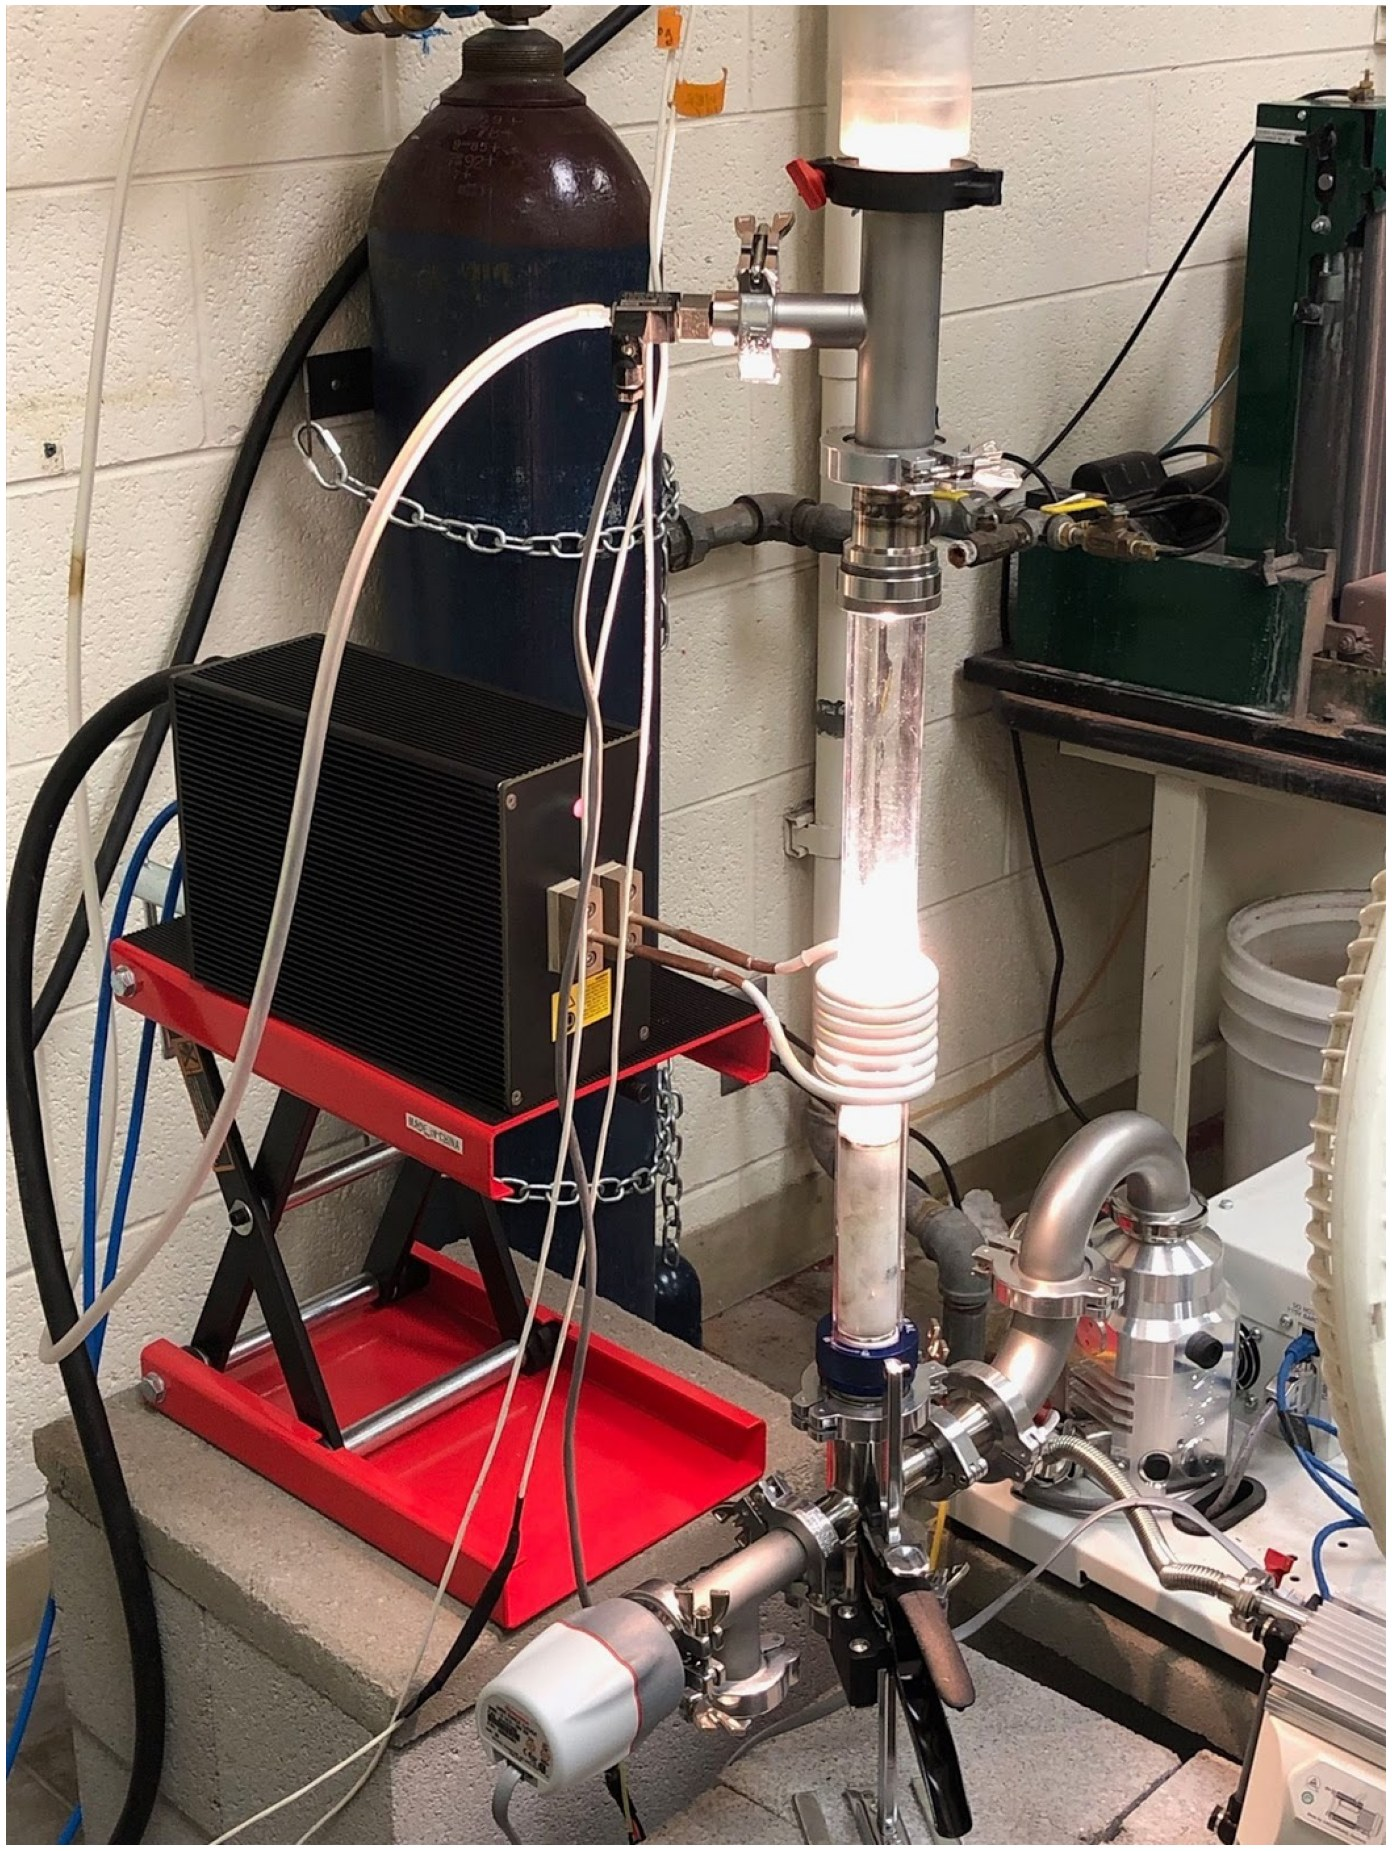
\includegraphics[width=0.8\linewidth]{fig_furnace_photo.jpg}
\caption{The fully assembled, functioning furnace. The heating head and work
coil, driven by the CEIA Power Cube generator, sit on the adjustable support
platform at left; the vertical quartz-tube vacuum chamber passes through the
coil and glows at the crucible position; the argon cylinder (rear) feeds the
gas-handling line; and the turbo pumping station connects at the lower right of
the chamber stack. Photograph contributed by R.~Guymon.}
\label{fig:furnacephoto}
\end{figure}

\paragraph{Heating path.} The generator's heating head, carrying the
water-cooled copper work coil ($\sim$3\,in tall, 2.5\,in ID, $\sim$6.5 turns;
drawing in \texttt{docs/coils-drawing.pdf}), mounts on an adjustable platform on
the bolted support stand (8 short + 4 long sections, 12 corner braces, 4 floor
mounts) so the coil can be centered on the crucible position of the vertically
mounted quartz tube. The recirculating chiller supplies cooling water to the
generator and coil, which carry both the RF current and the coolant. \todo{state
the exact copper-tube OD/wall, bend radius/spacing method, and
cooling-connection fittings from the coil drawing (docs/coils-drawing.pdf).}
Inside the tube, the machined graphite crucible/susceptor
(Figs.~\ref{fig:crucible}--\ref{fig:crucible-assembly}), machined from
3000\,\celsius{} graphite stock and repaired with graphite cement when cracked,
seats at coil height on a ceramic-cylinder/Teflon spacer stack; the pyrometer,
held by a stand-mounted holder, sights the specimen through the optical window
and the sapphire disc in the crucible lid.

\paragraph{Vacuum path.} The chamber is the fused-quartz tube itself. Its open
end terminates in a KF40 flange whose optical window --- a 55\,mm quartz disc
seated on the overpressure centering ring and held by a reusable plastic
quick-clamp (a Torr-Seal'd blank flange is the documented permanent-seal
alternative) --- closes the top of the stack. From the bottom of the chamber
stack, a tee carries a 0.5\,psi overpressure relief valve
(Fig.~\ref{fig:vacuumdetails}(b)) that protects the quartz tube from accidental
overpressure during backfilling, and a flexible stainless bellows continues
through the wide-range vacuum gauge to the Edwards T-Station~85 turbo pumping
station. The roughing pump sits on a separate support, mechanically decoupled
from the vacuum-chamber attachment tubes, so its vibration does not reach the
chamber and the pyrometer sight line (Fig.~\ref{fig:vacuumdetails}(a)).

\paragraph{Gas path.} The argon cylinder regulator feeds a digital mass flow
controller (Sierra Smart-Trak; Fig.~\ref{fig:vacuumdetails}(c)) whose metered
output connects to the manual vent valve, providing both controlled venting and
low-flow inert backfilling of the chamber; the LabVIEW front panel exposes the
flow setpoint and readback (Fig.~\ref{fig:controlpanel}).

\paragraph{Control path.} The DAQ's 0--5\,V analog output drives the
voltage-to-current loop conditioner, whose 4--20\,mA output lands on the CEIA
Power Controller's analog power-setpoint input (the LEPEL prototype took a
0--5\,mA command directly); the pyrometer's analog output returns to a DAQ
analog input, scaled to \celsius{} (wiring details in
\texttt{docs/temp-control-modification/}). Electrical isolation is maintained
between the DAQ/control path and the generator interface throughout. The
LabVIEW VIs from \texttt{code/} are deployed against these DAQ channels, and
manual control is verified before automated ramp/soak is enabled.

\begin{figure*}[ht]
\centering
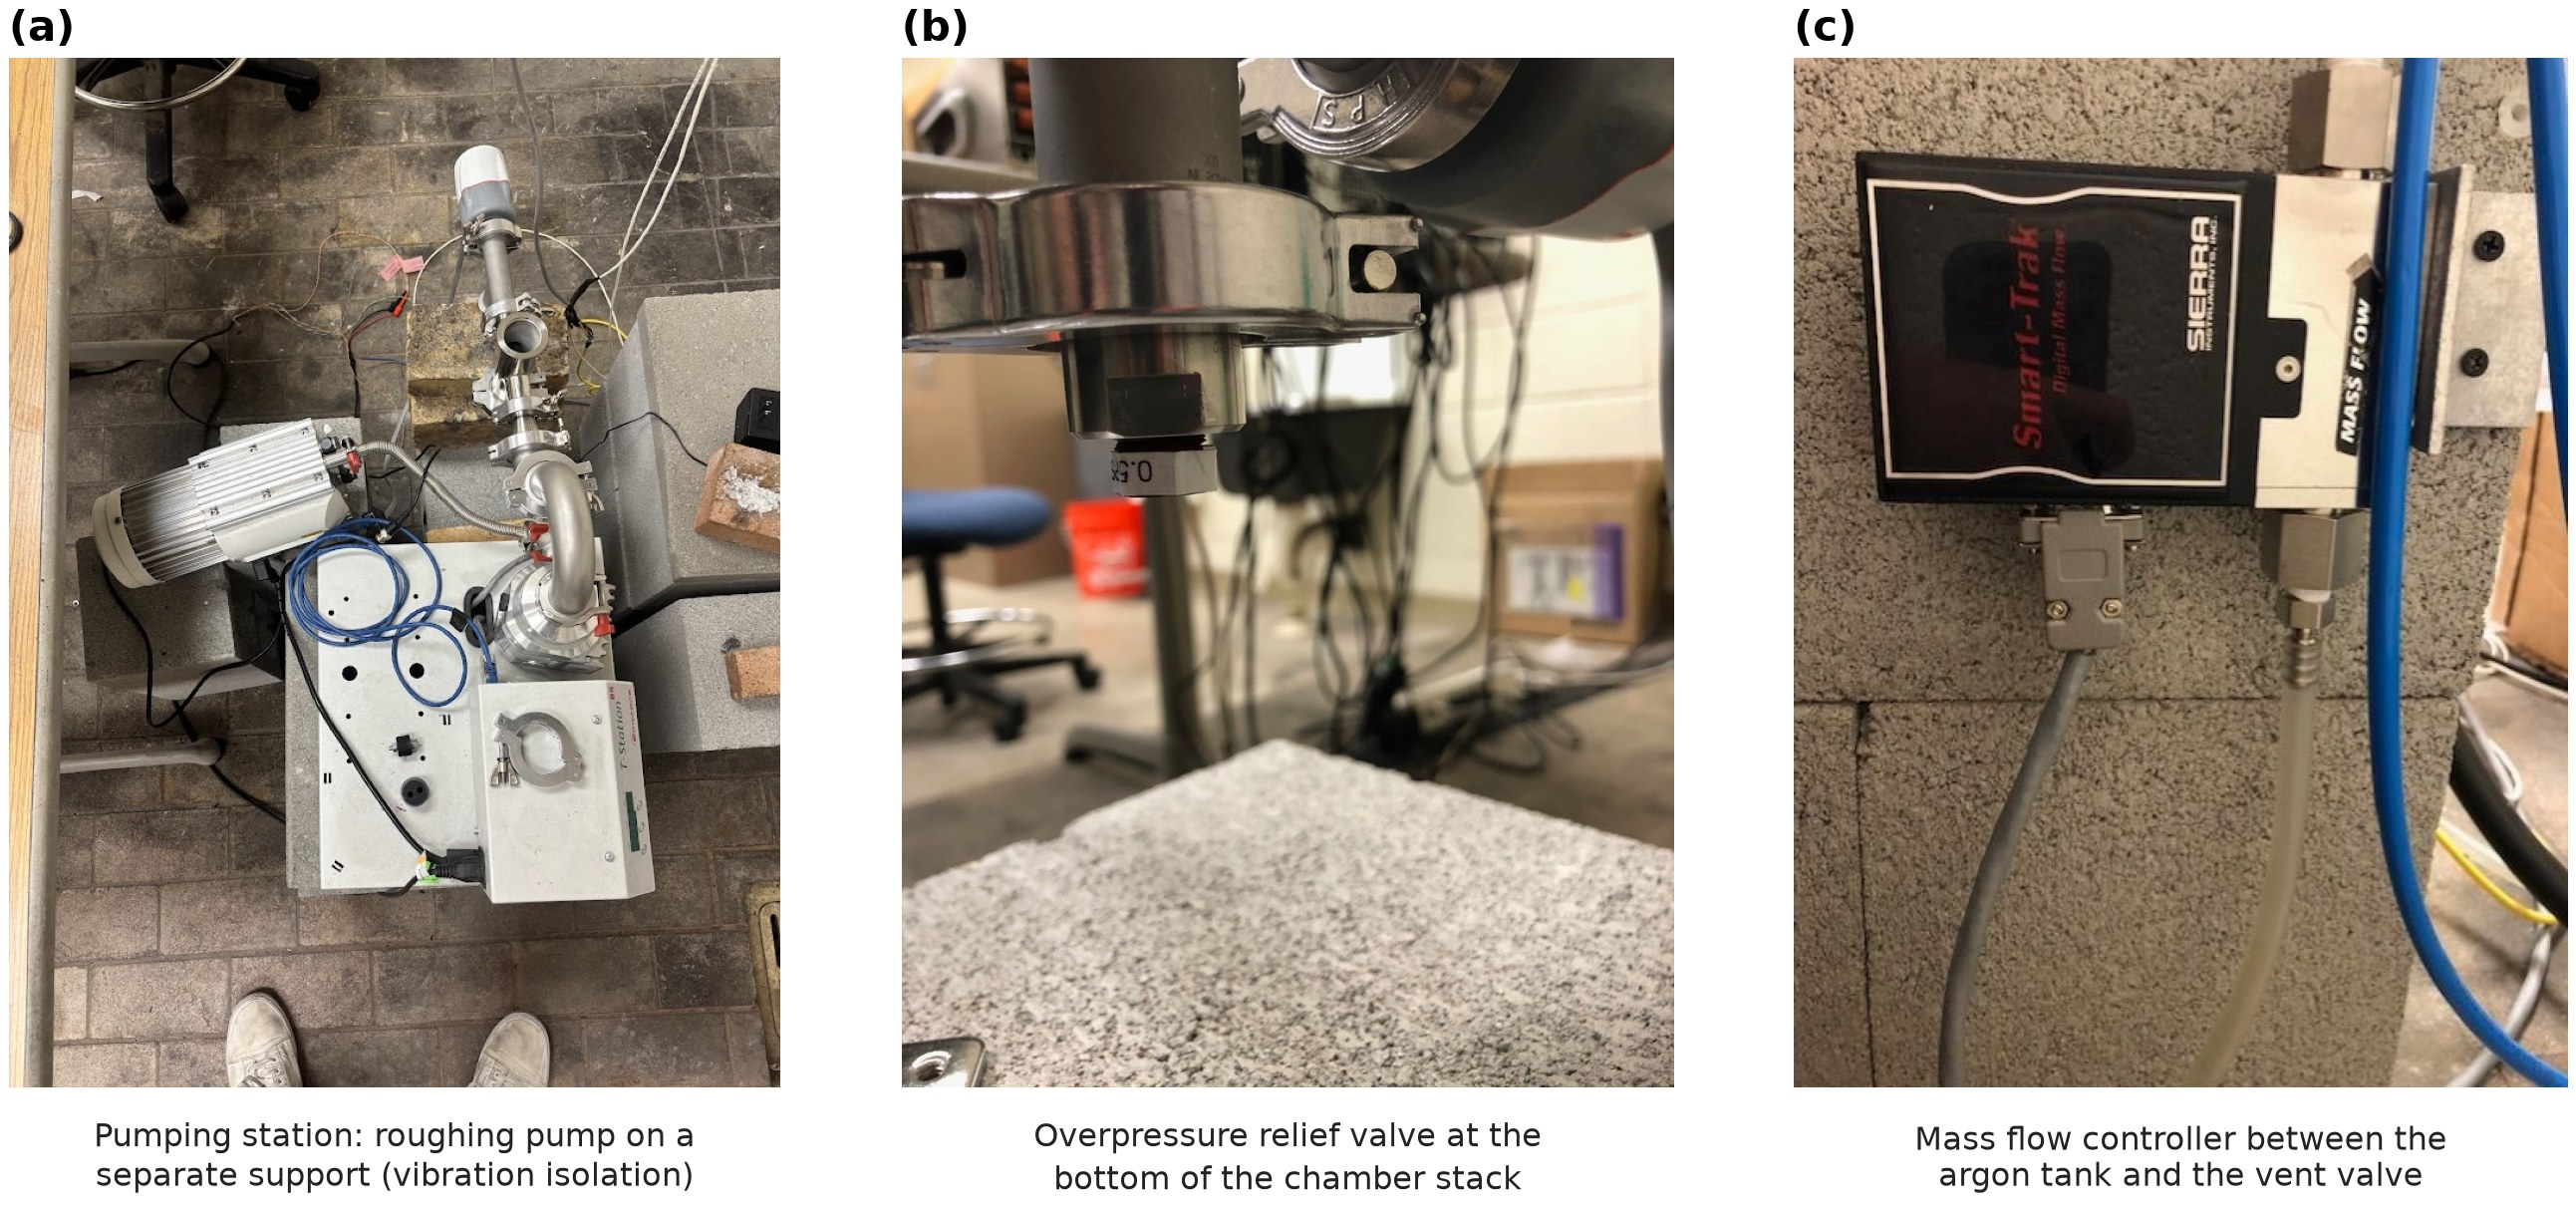
\includegraphics[width=0.92\linewidth]{fig_vacuum_details.jpg}
\caption{Vacuum and gas-handling details of the assembled system.
(a)~Turbo pumping station with the roughing pump mounted on a separate support,
not connected to the vacuum-chamber attachment tubes, so pump vibration is not
transmitted into the chamber (chamber shown disassembled).
(b)~Overpressure relief valve (0.5\,psi cracking pressure) at the bottom of the
vacuum chamber stack. (c)~Digital mass flow controller (Sierra Smart-Trak)
connecting the argon tank to the vent valve for controlled venting and inert
backfill. Photographs contributed by R.~Guymon.}
\label{fig:vacuumdetails}
\end{figure*}

\subsection{Operating procedure}

The operating procedure below is condensed from the lab SOP
(\texttt{extracted-context/SOP\_induction\_200901.md}). Before RF power is ever
applied, the chamber must be at high vacuum
($\sim$1$\times$10$^{-6}$\,Torr or better) or backfilled to the intended inert
atmosphere; cooling-water flow at the coil and generator must be confirmed and
leak-free; the coil, sample, and pyrometer sight line must be aligned; and all
conductive objects (jewelry, watches, phones, tools) must be at least
6--12\,in from the coil.

A run begins with the chamber vented to atmosphere --- the vent valve is never
opened while the turbo pump is spinning. The specimen is loaded into the
graphite crucible (Fig.~\ref{fig:crucible-assembly}), the crucible/spacer stack
is inserted into the quartz tube, and the KF40 flange is clamped finger-tight on
its O-ring. With the vent valve closed, the roughing and turbo pumps are brought
up and the chamber pumped to high vacuum. The generator is then powered on per
its own startup sequence and the LabVIEW ramp/soak profile started. Below the
pyrometer's $\sim$700\,\celsius{} detection floor the VI ramps open-loop on the
analog command; once the pyrometer returns a sustained valid reading above that
floor, control hands over to closed-loop PID on the optical temperature, and the
programmed profile (e.g., $\sim$1200\,\celsius{} for several hours for Ni grain
growth) runs to completion, with optional email status alerts from the VI. At
the end of the profile, power ramps down and RF stops; the sample cools under
vacuum, and the chamber is vented only after the turbo pump has fully stopped.

Off-normal conditions all call for removing RF power first. On loss of cooling
water or a chiller alarm, the analog command is zeroed immediately and the
generator not re-energized until flow is restored. On vacuum loss or a
quartz-tube fracture, RF is stopped immediately and the chamber is never vented
against a spinning turbo pump. On arcing, smoke, or runaway temperature, the
command is zeroed, RF is killed at the generator, and the system is locked out
before inspection.

\subsection{Safety}

The system combines RF power, high vacuum, high temperature, and cooling water,
and each pairing carries its own hazard. The energized coil can shock or burn
through direct contact or through currents induced in nearby conductors, so
conductive objects and electronics are kept at least 6--12\,in away, the
DAQ/control path is electrically isolated from the generator interface, and any
service inside the generator follows lockout/tagout. The evacuated quartz tube
poses a fracture/implosion risk --- operators wear safety glasses --- and
venting against a spinning turbo pump can destroy the pump, so the turbo must
spin down fully before the vent valve opens. Because the coil and chiller run
water immediately next to energized hardware, flow is confirmed and leaks are
checked before RF is applied, and water lines are routed away from electronics.
A melted-through specimen or hot graphite oxidizing on a premature vent can
contaminate the pump line and burn the operator, so samples cool under vacuum
and vacuum components are handled with clean nitrile gloves. Inert-gas
backfilling in an enclosed space is an asphyxiation risk and is done only with
adequate ventilation. Finally, the RF near-field can corrupt or damage nearby
instruments, which are shielded and kept clear of the coil.

%==============================================================
\section{Performance validation}
%==============================================================

The repository contains 100+ logged runs (\texttt{docs/data\_log/}, IFrun001--100)
across Ni200, Ni4N5, YSZ, and Pd thermal-evaporation experiments, with temperatures
of $\sim$900--1400\,\celsius{} and soak durations from minutes to $\sim$40\,h, each
with \texttt{.xlsx}/\texttt{.txt}/\texttt{.lvm} traces and some photos. Per-run traces
were parsed into uniform CSV/PNG files (\texttt{docs/data\_log/processed/};
\texttt{build\_run\_traces.py}), and the quantitative metrics below were computed
reproducibly from those traces by \texttt{paper/build\_validation\_figures.py}
(values mirrored in \texttt{paper/validation-metrics.json}). Because the archive is a
retrospective operating record rather than a prospectively balanced design of
experiments, every comparison is restricted to an internally consistent subset
(matching material, nominal profile, and operating configuration) and the
power--temperature relation is reported as an \emph{operational}
calibration for one fixed geometry, not as a universal transfer function.

\paragraph{Power-command $\rightarrow$ temperature calibration
(Fig.~\ref{fig:calibration}).} For one fixed Ni4N5/quartz/graphite/optical
configuration, four archived steady-state anneals spanning 1200--1400\,\celsius{}
(\texttt{IFrun039}, \texttt{IFrun040}, \texttt{IFrun038}, \texttt{IFrun032}) give a
monotonic relation between the soak-mean analog power command and the soak-mean
pyrometer temperature. A linear guide-to-the-eye fit over these points is
$T \approx 931 + 632\,I$ (\celsius, $I$ in mA), $R^2 = 0.991$, $n = 4$. This is
presented as an operational calibration only: the broader archive shows
configuration-dependent offsets (e.g.\ runs near 1200\,\celsius{} required soak-mean
commands of $\sim$0.44\,mA vs.\ $\sim$0.66\,mA in a different era/geometry), so the
fit must not be read as a universal command--temperature law.

\begin{figure}[ht]
\centering
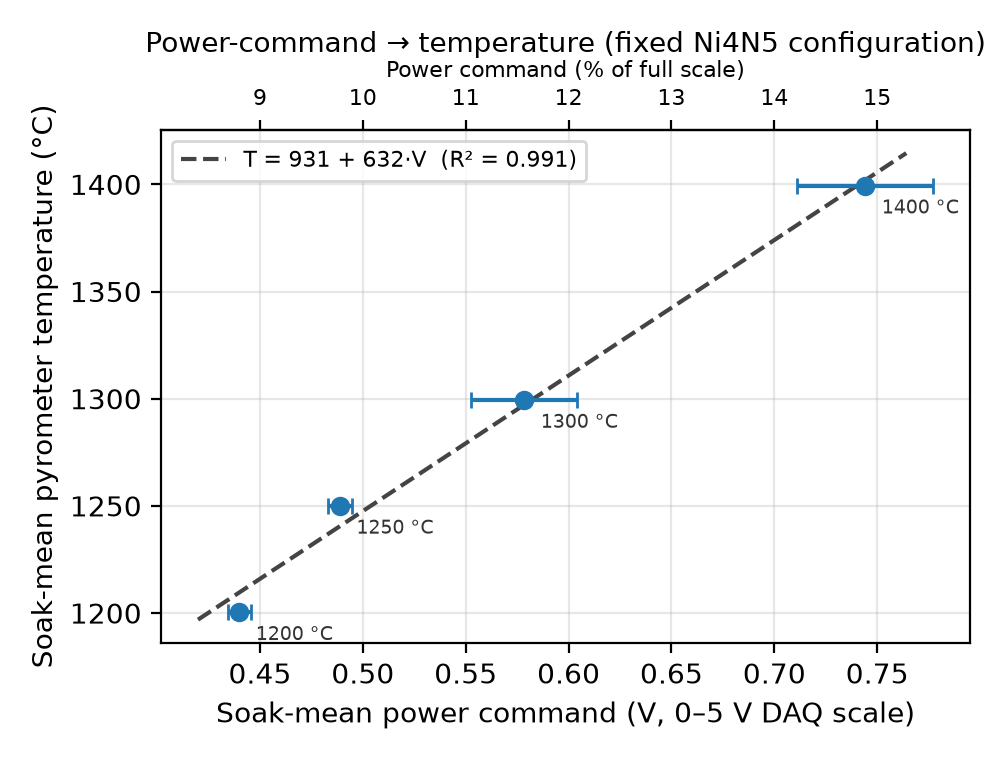
\includegraphics[width=0.72\linewidth]{fig_calibration.png}
\caption{Power-command $\rightarrow$ temperature calibration for one fixed archived
Ni4N5 configuration. Points are soak-mean values; horizontal bars are the in-soak SD
of the analog command. The dashed line is a guide-to-the-eye linear fit
($R^2 = 0.991$, $n = 4$).}
\label{fig:calibration}
\end{figure}

\paragraph{Representative ramp/soak with control metrics
(Fig.~\ref{fig:representative}).} Run \texttt{IFrun079\_Ni4N5\_084\_1300C\_12h} is a
representative closed-loop anneal. Measured against the 1300\,\celsius{} setpoint, the
soak held $1302.1 \pm 3.0$\,\celsius{} (mean\,$\pm$\,SD) over the 12\,h plateau, with a
10--90\,\% rise time of $\sim$1135\,s, an overshoot of $\sim$12\,\celsius, a maximum
in-soak deviation of $\sim$10\,\celsius, and a near-zero linear drift of
$-0.02$\,\celsius/h, demonstrating that the pyrometer-feedback loop holds a programmed
soak over many hours.

\begin{figure}[ht]
\centering
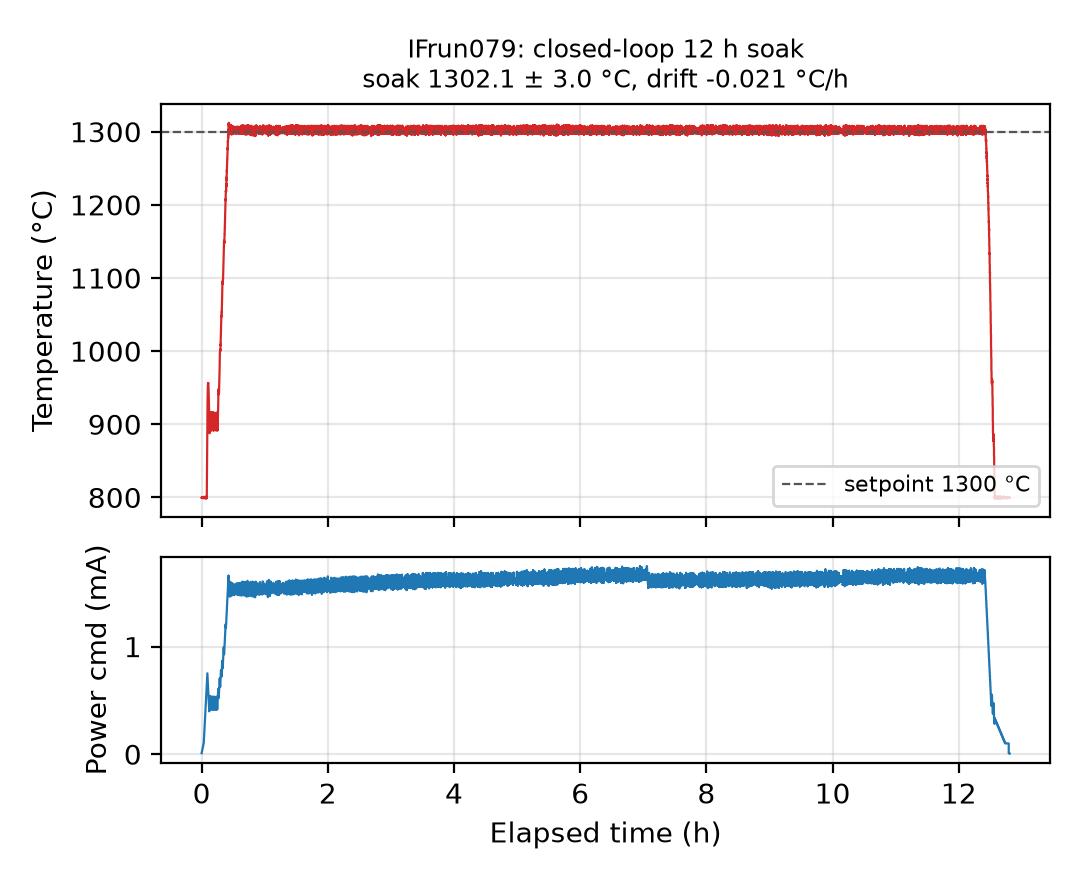
\includegraphics[width=0.78\linewidth]{fig_representative.png}
\caption{Representative closed-loop anneal (\texttt{IFrun079}, Ni4N5, nominal
1300\,\celsius{} / 12\,h): pyrometer temperature with setpoint overlay (top) and analog
power command (bottom). Soak mean $1302.1 \pm 3.0$\,\celsius, drift $-0.02$\,\celsius/h.}
\label{fig:representative}
\end{figure}

\paragraph{Repeatability and long-soak stability
(Figs.~\ref{fig:repeatability}--\ref{fig:longsoak}).} Run-to-run repeatability was
assessed on the most internally consistent cohort available: eight Ni4N5 anneals at a
nominal 1200\,\celsius{} / 12\,h condition (\texttt{IFrun052}--\texttt{IFrun060},
excluding missing run numbers), all logged under the same gas-flow configuration.
Across these runs the soak temperature was $1201.2 \pm 1.3$\,\celsius{}
(range 1199.8--1204.2\,\celsius; coefficient of variation 0.11\,\%; $n = 8$), peak
temperature $1212.6 \pm 6.7$\,\celsius, and soak duration $766 \pm 15$\,min. Runs from
other periods or geometries (e.g.\ \texttt{IFrun016}, \texttt{IFrun019},
\texttt{IFrun049}) are deliberately \emph{not} pooled into this estimate. Long-duration
stability was demonstrated with two Ni200 anneals at 1325\,\celsius: a 20\,h run
(\texttt{IFrun081}) held $1326.5 \pm 1.5$\,\celsius{} with drift $-0.004$\,\celsius/h,
and a 40\,h run (\texttt{IFrun080}) maintained $\sim$1326--1329\,\celsius{} over
2400\,min in-band.

\begin{figure}[ht]
\centering
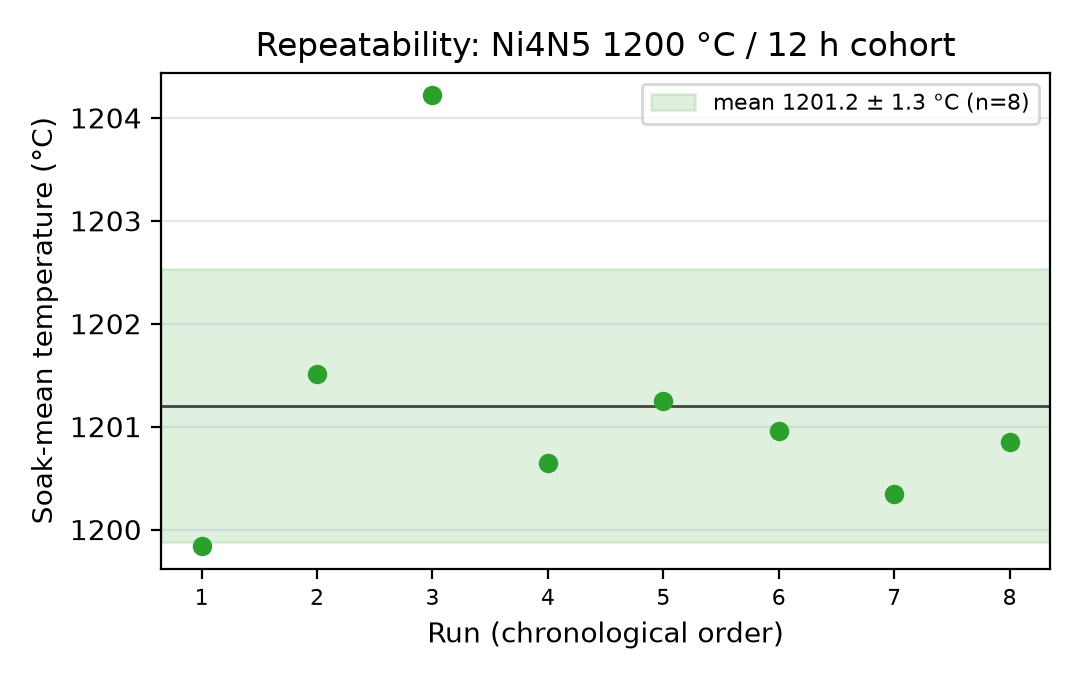
\includegraphics[width=0.74\linewidth]{fig_repeatability.png}
\caption{Run-to-run repeatability of the Ni4N5 1200\,\celsius{} / 12\,h cohort
(\texttt{IFrun052}--\texttt{IFrun060}, $n = 8$). Points are per-run soak-mean
temperatures; the band is mean\,$\pm$\,SD ($1201.2 \pm 1.3$\,\celsius).}
\label{fig:repeatability}
\end{figure}

\begin{figure}[ht]
\centering
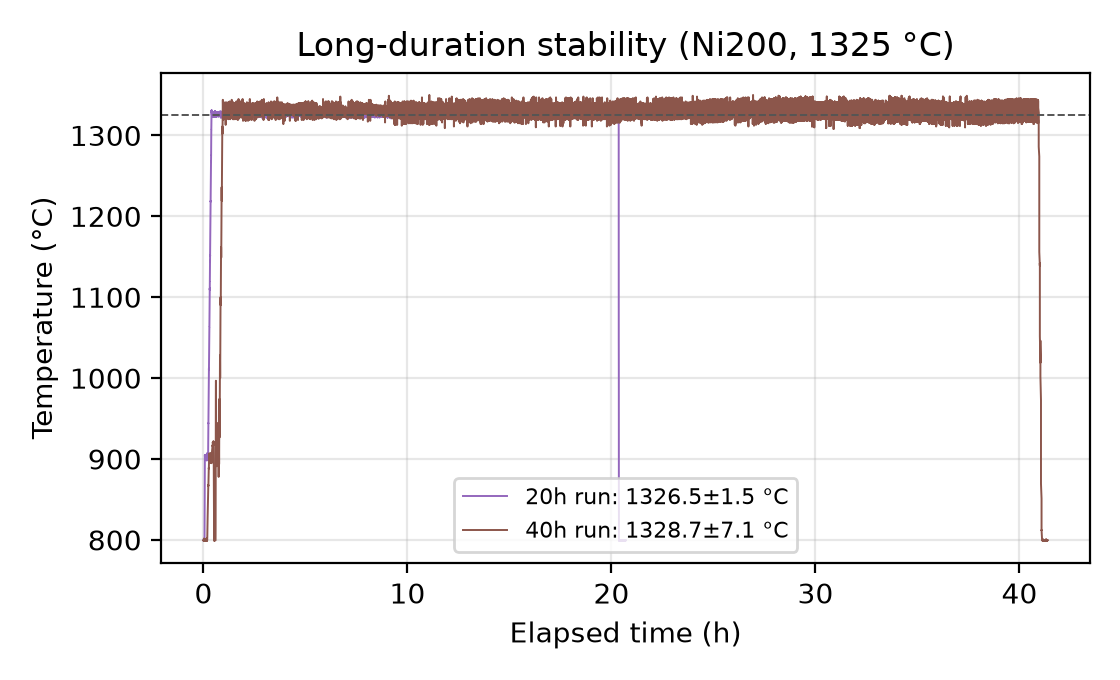
\includegraphics[width=0.78\linewidth]{fig_longsoak.png}
\caption{Long-duration thermal stability: Ni200 anneals at 1325\,\celsius{} held for
20\,h (\texttt{IFrun081}) and 40\,h (\texttt{IFrun080}).}
\label{fig:longsoak}
\end{figure}

%==============================================================
\section{Microstructural validation}
%==============================================================

The furnace exists to change microstructure, so the key validation is
\textbf{real microstructural data} tied to specific thermal histories. The
committed SEM/EBSD and optical-microscopy archives (\texttt{docs/SEM/},
\texttt{docs/optical/}) are keyed by \texttt{Ni4N5\_\#\#\#} /
\texttt{Ni200\_\#\#\#} specimen IDs that map directly
to the run IDs in \texttt{docs/data\_log/}. This mapping is built reproducibly by
\texttt{paper/build\_characterization\_crossref.py}, which parses the specimen ID
out of every characterization folder, joins it to the machine-parsed run summary,
and writes the per-specimen cross-reference in
\texttt{paper/characterization-crossref.csv}/\texttt{.md}: \textbf{35 characterized
specimens}, of which \textbf{9 link to a parsed run log}, \textbf{8 carry committed
EBSD/OIM data}, and one carries EDS. Inverse-pole-figure (IPF) EBSD orientation
maps of two annealed specimens (Fig.~\ref{fig:ebsd}) resolve hundreds of indexed
grains, and the best-correlated specimen, \texttt{Ni4N5\_081} (annealed in
\texttt{IFrun082} at a nominal 1300\,\celsius{} for 20\,h; logged soak
$\sim$1301\,\celsius), is documented across length scales --- optical grain map
with in-image grain-size measurements, SEM survey, and high-magnification
grain-boundary detail (Fig.~\ref{fig:microstructure}). The full multi-gigabyte
raster/EBSD archive (including \texttt{.oim}, \texttt{.osc}, \texttt{.ang}, and
DREAM.3D volumes) remains on the lab's Box share and is inventoried per file in
\texttt{docs/SEM/CATALOG.csv} and \texttt{docs/optical/CATALOG.csv}.
Grain size is quantified with: number of grains analyzed,
equivalent-circle-diameter or intercept metric, median + IQR (or mean $\pm$ SD),
segmentation/cleanup criteria, minimum-grain-area threshold, and whether twins are
merged or separated, with the specimen/run (not the individual grain) treated as the
experimental unit~\cite{liu2021studyofgrain,alogab2007theinfluenceof}. Where as-received baselines are unavailable for a batch, results are
framed as final-state comparisons across archived anneals rather than as fully
parameterized grain-growth kinetics.

\begin{figure}[ht]
\centering
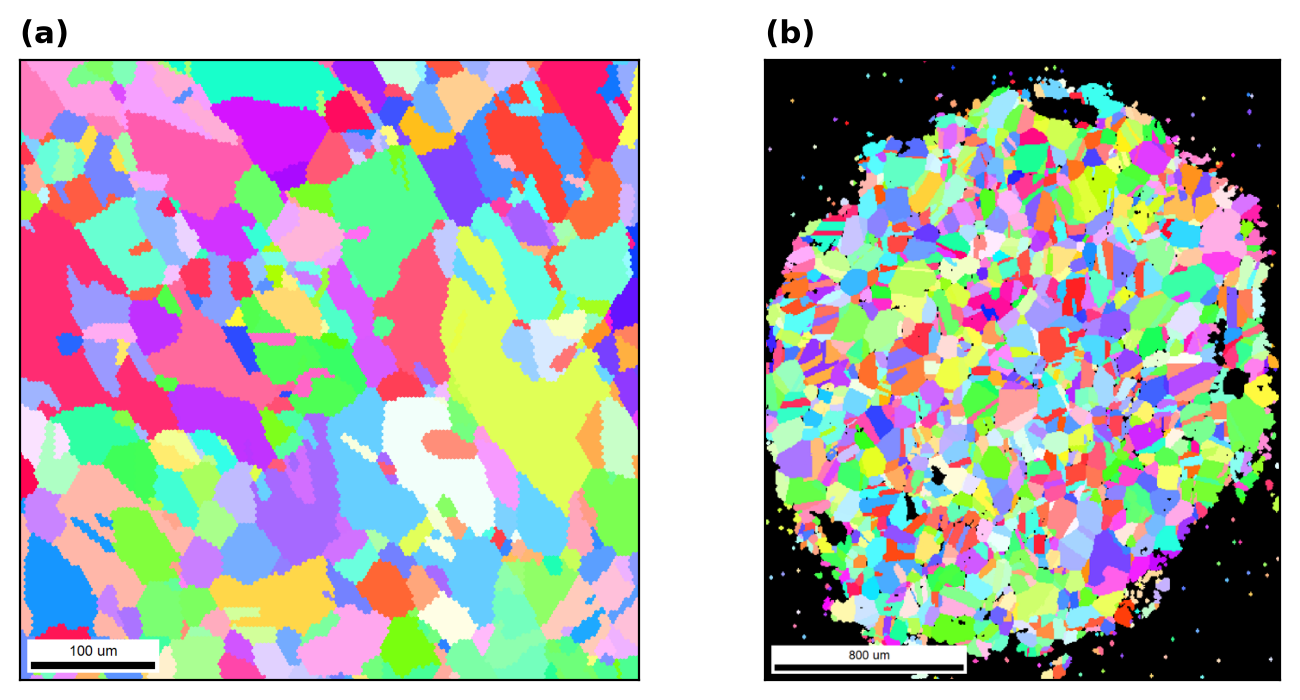
\includegraphics[width=0.86\linewidth]{fig_ebsd.png}
\caption{EBSD inverse-pole-figure (IPF) orientation maps of two annealed Ni4N5
specimens, rendered from the committed \texttt{docs/SEM/} archive.
(a)~\texttt{Ni4N5\_034} (\texttt{IFrun049}, 1200\,\celsius{} / 12\,h);
(b)~\texttt{Ni4N5\_069}. Each indexed color is a crystallographic orientation;
the maps resolve hundreds of grains for grain-size and texture analysis.}
\label{fig:ebsd}
\end{figure}

\begin{figure*}[ht]
\centering
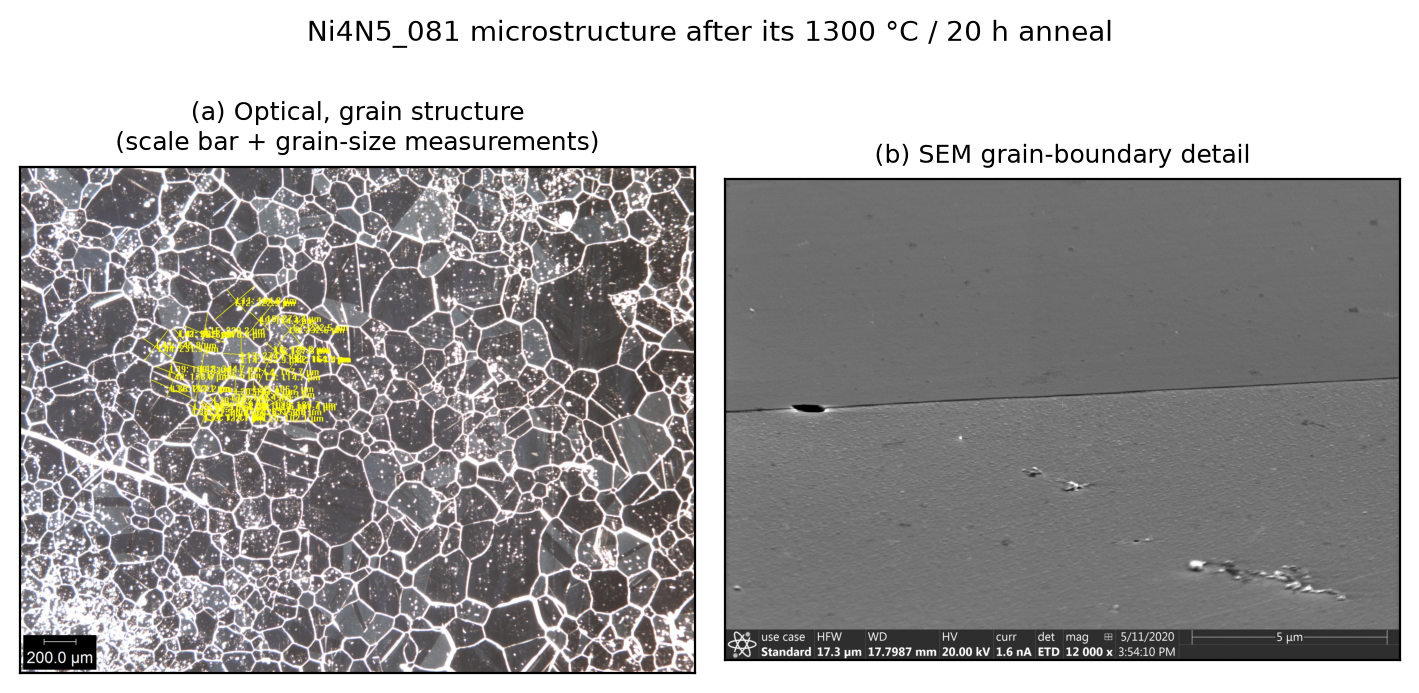
\includegraphics[width=0.96\linewidth]{fig_microstructure.png}
\caption{Multi-scale microstructure of specimen \texttt{Ni4N5\_081} after
\texttt{IFrun082} (nominal 1300\,\celsius{} / 20\,h, gas flow), correlating the
characterization archive with a single logged thermal history.
(a)~Optical micrograph (grain structure, 200\,\textmu m scale bar, with in-image
grain-size measurements); (b)~SEM survey; (c)~high-magnification SEM
grain-boundary detail. All panels are committed files under \texttt{docs/optical/}
and \texttt{docs/SEM/}.}
\label{fig:microstructure}
\end{figure*}

Controls that further isolate the instrument's behavior --- open-loop vs.\
closed-loop on the same target cycle, vacuum vs.\ inert-gas backfill mode,
directly-coupled metal vs.\ susceptor-mediated ceramic heating, and multi-hour
long-soak stability --- are partially represented in the archive and are natural
extensions for a prospective study.

\paragraph{Specimen $\leftrightarrow$ thermal-history linkage.} Each microstructure
specimen is tied to its exact run via Table~\ref{tab:linkage}. ``Nominal soak'' is the
target parsed from the run filename; ``logged soak T'' is the machine-parsed soak-mean
from the trace (\texttt{run\_summary.csv}); ``atmosphere'' indicates whether active gas
flow was present in the parsed log summary (\texttt{has\_flow}), not a fully
reconstructed gas chemistry.

\begin{table*}[ht]
\caption{Specimen $\leftrightarrow$ thermal-history linkage for the runs used in
the validation figures.
\label{tab:linkage}}
\scriptsize
\setlength{\tabcolsep}{3pt}
\begin{tabularx}{\linewidth}{l l L{0.22\linewidth} R{0.06\linewidth} R{0.07\linewidth} l l X}
\toprule
\textbf{Specimen} & \textbf{Material} & \textbf{Run ID} & \textbf{Nominal soak} & \textbf{Logged soak T} & \textbf{Soak time} & \textbf{Atmosphere} & \textbf{Role / figure} \\
\midrule
Ni4N5\_026 & Ni4N5 & IFrun039\_Ni4N5\_026\_1200C\_6h & 1200\,\celsius & 1200.4\,\celsius & 6\,h & no-flow & Calibration (Fig.~\ref{fig:calibration}) \\
Ni4N5\_027 & Ni4N5 & IFrun040\_Ni4N5\_027\_1250C\_6h & 1250\,\celsius & 1250.0\,\celsius & 6\,h & no-flow & Calibration \\
Ni4N5\_025 & Ni4N5 & IFrun038\_Ni4N5\_025\_1300C\_1h & 1300\,\celsius & 1299.9\,\celsius & 1\,h & no-flow & Calibration \\
Ni4N5\_022 & Ni4N5 & IFrun032\_Ni4N5\_022\_1400C\_10min & 1400\,\celsius & 1399.6\,\celsius & 10\,min & no-flow & Calibration \\
Ni4N5\_084 & Ni4N5 & IFrun079\_Ni4N5\_084\_1300C\_12h & 1300\,\celsius & 1302.1\,\celsius & 12\,h & flow & Representative (Fig.~\ref{fig:representative}) \\
Ni4N5\_040 & Ni4N5 & IFrun052\_Ni4N5\_040\_1200C\_12h & 1200\,\celsius & 1199.8\,\celsius & 12\,h & flow & Repeatability (Fig.~\ref{fig:repeatability}) \\
Ni4N5\_042,044 & Ni4N5 & IFrun054\_Ni4N5\_042,044\_1200C\_12h & 1200\,\celsius & 1201.5\,\celsius & 12\,h & flow & Repeatability \\
Ni4N5\_045,046 & Ni4N5 & IFrun055\_Ni4N5\_045,046\_1200C\_12h & 1200\,\celsius & 1204.2\,\celsius & 12\,h & flow & Repeatability \\
Ni4N5\_047,048 & Ni4N5 & IFrun056\_Ni4N5\_047,048\_1200C\_12h & 1200\,\celsius & 1200.6\,\celsius & 12\,h & flow & Repeatability \\
Ni4N5\_049,050 & Ni4N5 & IFrun057\_Ni4N5\_049,050\_1200C\_12h & 1200\,\celsius & 1201.2\,\celsius & 12\,h & flow & Repeatability \\
Ni4N5\_051,052 & Ni4N5 & IFrun058\_Ni4N5\_051,052\_1200C\_12h & 1200\,\celsius & 1201.0\,\celsius & 12\,h & flow & Repeatability \\
Ni4N5\_053,054 & Ni4N5 & IFrun059\_Ni4N5\_053,054\_1200C\_12h & 1200\,\celsius & 1200.3\,\celsius & 12\,h & flow & Repeatability \\
Ni4N5\_056,057 & Ni4N5 & IFrun060\_Ni4N5\_056,057\_1200C\_12h & 1200\,\celsius & 1200.9\,\celsius & 12\,h & flow & Repeatability \\
Ni200\_015 & Ni200 & IFrun081\_Ni200\_015\_1325C\_20h & 1325\,\celsius & 1326.5\,\celsius & 20\,h & flow & Long soak (Fig.~\ref{fig:longsoak}) \\
Ni200\_017 & Ni200 & IFrun080\_Ni200\_017\_1325C\_40h & 1325\,\celsius & 1326.3\,\celsius & 40\,h & flow & Long soak \\
Ni4N5\_079,080 & Ni4N5 & IFrun072\_Ni4N5\_079,080\_1400C\_12h & 1400\,\celsius & --- & 12\,h & flow & Process-window specimen \\
\bottomrule
\end{tabularx}
\end{table*}

\paragraph{Characterization $\leftrightarrow$ run inventory.}
Table~\ref{tab:charxref} lists the specimens that carry committed
SEM/EBSD/optical data \emph{and} a matched parsed run log (generated by
\texttt{paper/build\_characterization\_crossref.py}). Two specimens
(\texttt{Ni4N5\_034}, \texttt{Ni4N5\_081}) carry committed EBSD orientation maps
on top of SEM/optical imaging, and \texttt{Ni4N5\_081} is the most completely
characterized run (Fig.~\ref{fig:microstructure}). The complete 35-specimen
cross-reference, including characterized specimens whose run logs are not in the
parsed set, is in \texttt{paper/characterization-crossref.csv}.

\begin{table}[ht]
\caption{Specimens with committed characterization data and a matched, parsed
furnace run. ``SEM''/``Opt.'' are committed file counts; ``EBSD'' flags committed
inverse-pole-figure/OIM data. Full inventory in
\texttt{paper/characterization-crossref.csv}.
\label{tab:charxref}}
\scriptsize
\setlength{\tabcolsep}{4pt}
\begin{tabular}{l l l r r c}
\toprule
\textbf{Specimen} & \textbf{Material} & \textbf{Matched run} & \textbf{SEM} & \textbf{Opt.} & \textbf{EBSD} \\
\midrule
Ni200\_001 & Ni200 & IFrun004/005 & 0 & 3 & no \\
Ni200\_015 & Ni200 & IFrun081 (1325\,\celsius/20\,h) & 0 & 3 & no \\
Ni200\_017 & Ni200 & IFrun080 (1325\,\celsius/40\,h) & 0 & 2 & no \\
Ni4N5\_001b & Ni4N5 & IFrun006 & 0 & 2 & no \\
Ni4N5\_010 & Ni4N5 & IFrun016 (1200\,\celsius) & 0 & 4 & no \\
Ni4N5\_012 & Ni4N5 & IFrun019 (1200\,\celsius) & 0 & 1 & no \\
Ni4N5\_034 & Ni4N5 & IFrun049 (1200\,\celsius/12\,h) & 4 & 0 & \textbf{yes} \\
Ni4N5\_053 & Ni4N5 & IFrun059 (1200\,\celsius/12\,h) & 3 & 3 & no \\
Ni4N5\_081 & Ni4N5 & IFrun082 (1300\,\celsius/20\,h) & 10 & 10 & \textbf{yes} \\
\bottomrule
\end{tabular}
\end{table}

\subsection{Extension to ceramic charges: YSZ}
\label{sec:ysz}

The same control, vacuum, and sensing stack extends to charges that do not
couple to the RF field at all, demonstrated with grain growth in
yttria-stabilized zirconia (YSZ). Ceramic grain growth requires substantially
higher soak temperatures ($\sim$1600--1700\,\celsius) than the Ni anneals ---
beyond the service range of the alumina spacers (1787\,\celsius{} rating) and
too hot for the graphite lid/sapphire-window geometry of
Fig.~\ref{fig:crucible-assembly} --- so only the charge stack inside the quartz
tube is exchanged (Fig.~\ref{fig:ysz}(a)). The YSZ specimen is sandwiched
between two tantalum blocks (25.5\,mm diameter) that replace graphite as the
susceptor at these temperatures; the pair seats in a MgO crucible (28\,mm) that
tolerates the higher temperature, and the crucible stands on an alumina support
rod that raises the stack to coil height inside a fresh $\sim$35\,mm-ID quartz
tube. The generator, vacuum path, gas handling, pyrometer, and LabVIEW control
are untouched --- the swap is a specimen-stack change, not a furnace change.
Committed optical micrographs from the characterization archive
(Fig.~\ref{fig:ysz}(b,c)) show the resulting equiaxed YSZ grain structures,
including a specimen after a 1700\,\celsius{} / 10\,h anneal. \todo{the
quantitative YSZ grain-growth dataset (anneal temperatures/times, grain-size
series) lives in a BYU Box folder whose shared link currently requires login
(byu.app.box.com/folder/298111707639); incorporate run conditions and grain-size
measurements, and confirm which archived YSZ anneals were performed in this
furnace, once the link is opened.}

\begin{figure*}[ht]
\centering
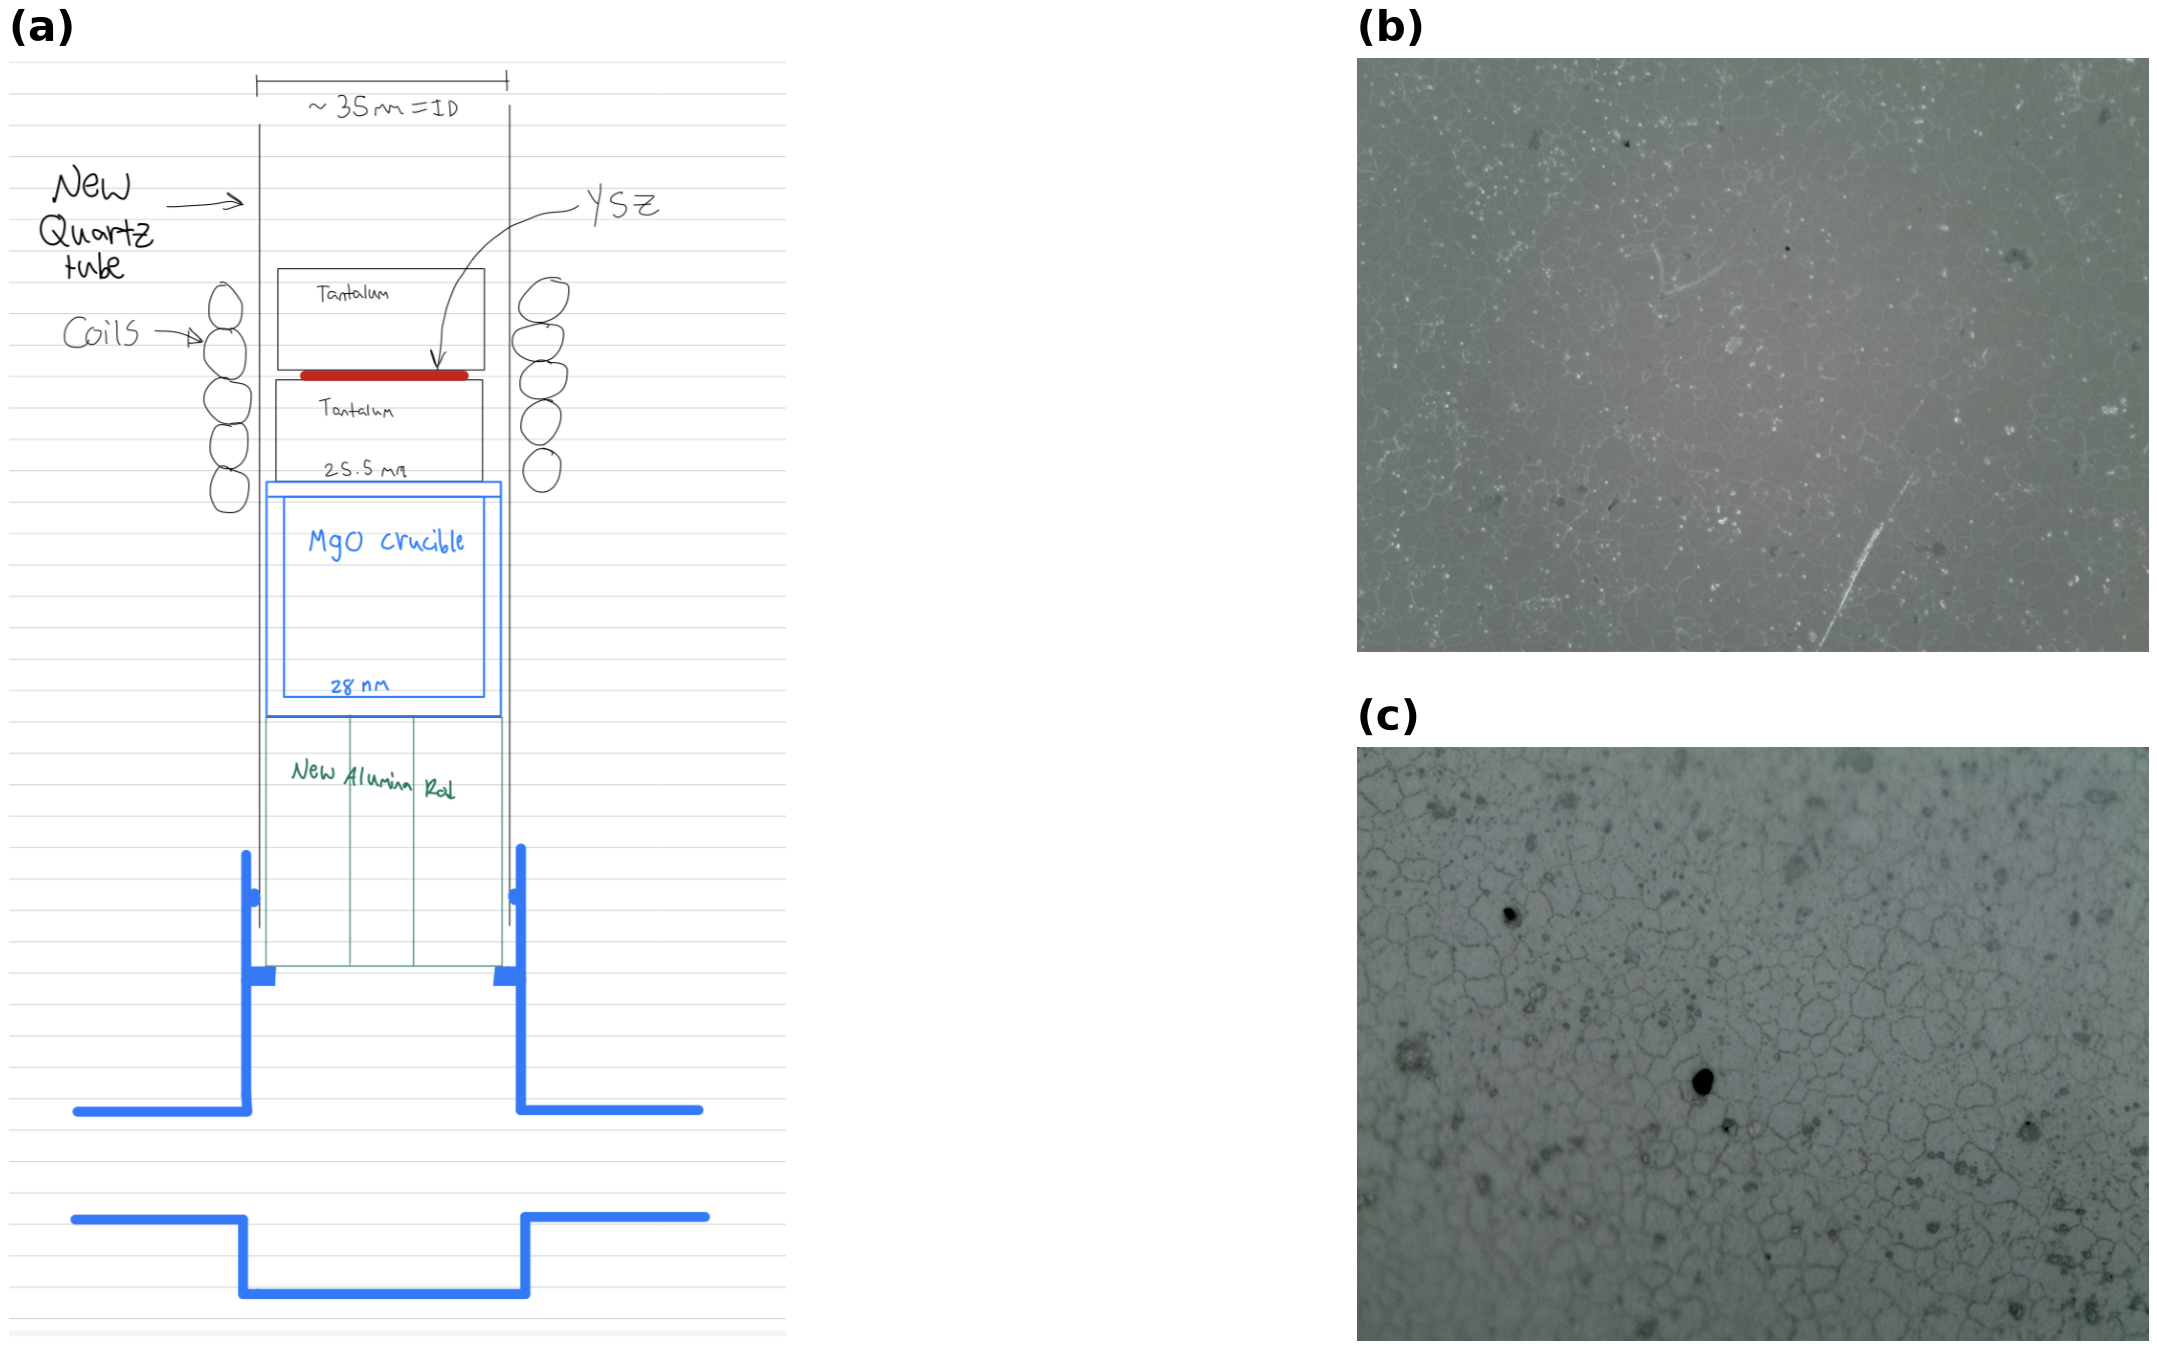
\includegraphics[width=0.92\linewidth]{fig_ysz.png}
\caption{High-temperature ceramic (YSZ) configuration and resulting
microstructure. (a)~Charge-stack schematic (contributed by R.~Guymon): inside a
fresh $\sim$35\,mm-ID quartz tube, the YSZ specimen (red) is sandwiched between
two 25.5\,mm tantalum susceptor blocks, seated in a 28\,mm MgO crucible on an
alumina support rod that raises the stack to coil height; the coil, vacuum,
pyrometer, and control paths are unchanged from the metal configuration.
(b)~Optical micrograph of YSZ after a 1700\,\celsius{} / 10\,h anneal
(\texttt{docs/optical/.../190823\_YSZ/YSZ\_1700C\_10h.JPG}).
(c)~Optical micrograph of an induction-annealed YSZ specimen
(\texttt{docs/optical/.../190909\_YSZ/}), showing the equiaxed grain structure;
scale-bar originals are inventoried in \texttt{docs/optical/CATALOG.csv}.}
\label{fig:ysz}
\end{figure*}

\subsection{Limitations of the retrospective validation}

The validation dataset is retrospective rather than prospectively designed, so the
archived runs are not treated as a balanced factorial experiment and comparisons are
restricted to internally consistent subsets. Because induction coupling, radiative view
factors, and pyrometer line-of-sight depend on specimen/crucible geometry and optical
alignment, the power-command/temperature calibration is reported only for a fixed
archived configuration and is not a universal transfer function. Reported temperatures
are closed-loop ratio-pyrometer readings in a fixed optical geometry; absolute specimen
temperature may still depend on emissivity and surface condition not fully
reconstructable for every archived run~\cite{ham2016insituspectralemissivity,suleiman2025improvingpyrometryof}.
Run-to-run repeatability is evaluated only within the most consistent cohort
(\texttt{IFrun052}--\texttt{IFrun060}); most other temperature/time conditions are
singletons, so inference is limited to descriptive summaries. Microstructural
comparisons are reported only for specimens whose image files link unambiguously to a
logged thermal history; ambiguously labeled images are excluded rather than inferred.

%==============================================================
\section{Conclusions}
%==============================================================

A bare commercial RF induction generator can be converted into a
computer-controlled, vacuum-integrated, pyrometer-feedback annealing system with a
documented, generator-agnostic modernization layer: LabVIEW/DAQ analog power
control, dual-wavelength optical temperature feedback, a high-vacuum quartz-tube
chamber, and an in-house machined graphite crucible/susceptor. Ported from a
$\sim$1970 LEPEL prototype to a current CEIA solid-state generator, the same stack
demonstrated an operational power--temperature calibration ($R^2 = 0.991$ over
1200--1400\,\celsius{} in a fixed geometry), run-to-run soak repeatability of
$1201.2 \pm 1.3$\,\celsius{} across eight nominally identical Ni4N5 anneals, and
stable closed-loop soaks up to 40\,h at 1325\,\celsius, with annealed-specimen
microstructures (SEM/EBSD/optical) cross-referenced to their logged thermal
histories. Exchanging the graphite crucible stack for a
tantalum-susceptor/MgO-crucible variant extends the same furnace to
non-coupling ceramic charges at $\sim$1700\,\celsius, demonstrated with YSZ
grain growth. Because the layer requires only a monotonic analog power-control input
from the generator, the design is directly reusable by other laboratories at a
small fraction of the cost of turn-key vacuum induction furnaces; complete design
files, the costed bill of materials (Appendix~\ref{app:bom}), control software,
and the full run-log and characterization archives are openly available.

%==============================================================
\section*{Supplementary Material}
%==============================================================

The development repository
(\url{https://github.com/vertical-cloud-lab/custom-induction-furnace}; archival
snapshot \href{https://doi.org/10.5281/zenodo.20878017}{10.5281/zenodo.20878017})
contains the complete supplementary material: LabVIEW control VIs and MATLAB
utilities (\texttt{code/}), system schematics and the coil drawing
(\texttt{docs/}), the standard operating procedure, the full parts list, the
100+ raw and machine-parsed anneal logs (\texttt{docs/data\_log/}), the SEM/EBSD
and optical characterization archives with per-file catalogs
(\texttt{docs/SEM/}, \texttt{docs/optical/}), and the scripts that reproduce
every figure and metric in this paper (\texttt{paper/}).

\begin{acknowledgments}
BYU Mechanical Engineering Department; the Johnson group; Kevin Cole.
\todo{funding sources.}
\end{acknowledgments}

\section*{Author Declarations}

\subsection*{Conflict of Interest}

The authors have no conflicts to disclose. \todo{confirm with all authors.}

\subsection*{Ethics Approval}

This work did not involve human participants, human data, or animal subjects;
ethics approval is not applicable.

\subsection*{Author Contributions}

\todo{confirm CRediT roles} --- provisional: \textbf{Sterling G. Baird:}
Conceptualization, Software, Investigation, Writing -- original draft.
\textbf{Kevin Cole:} Methodology, Resources, Supervision.
Additional authors to be confirmed.

\section*{Data Availability}

The data that support the findings of this study are openly available in the
development repository
\texttt{vertical-cloud-lab/custom-induction-furnace}
(\url{https://github.com/vertical-cloud-lab/custom-induction-furnace}); an
archival snapshot (design files, run logs, characterization data, and extracted
context) is deposited at Zenodo,
\href{https://doi.org/10.5281/zenodo.20878017}{https://doi.org/10.5281/zenodo.20878017}.

\appendix

%==============================================================
\section{Bill of materials}
\label{app:bom}
%==============================================================

% Outstanding co-author (R. Guymon) review corrections to specific BOM rows
% (exact NI DAQ/module models and prices, Edwards T-Station 85H variant price,
% wide-range gauge model, TAV5 price, pyrometer used price) are tracked in the
% pull-request review and will be folded in on the next BOM pass.
Table~\ref{tab:bom} itemizes the build. Groupings are denoted by the
designator prefix: \textbf{GEN} = induction generator + controller (the current USA
reproducible build; the legacy LEPEL is the prototype alternative, not a line item),
\textbf{RETRO} = the reproducible retrofit (control / vacuum / sensing) parts, and
\textbf{CONS} = consumables. Full vendor/price detail for the RETRO and CONS parts is
in \texttt{extracted-context/parts\_list.md} (extracted from
\texttt{docs/induction\_parts\_list.xlsx}).

\textbf{Costing conventions:} all costs are in \textbf{USD}; prices are the lab's
purchase records (quote year $\sim$2019--2021), several from used/surplus/eBay sources
as noted; shipping and tax are excluded unless stated. \textbf{The build instructions
and the bill of materials are canonical for the CEIA system only}; the legacy LEPEL
prototype and the rejected CYSI import path are documented in the text
(Sec.~\ref{sec:portability}), not here.

\begin{table*}[ht]
\caption{Bill of materials for the reproducible CEIA-anchored build (USD; see
costing conventions in the text).
\label{tab:bom}}
\scriptsize
\setlength{\tabcolsep}{3pt}
\begin{tabularx}{\linewidth}{l L{0.30\linewidth} c L{0.10\linewidth} R{0.07\linewidth} L{0.16\linewidth} L{0.09\linewidth}}
\toprule
\textbf{Desig.} & \textbf{Component} & \textbf{No.} & \textbf{Unit \$} & \textbf{Total} & \textbf{Source} & \textbf{Material} \\
\midrule
GEN-1 & CEIA ``Power Cube'' PW3-90/50 solid-state RF generator (V3000-0070) & 1 & \$8{,}240 & \$8{,}240 & East Coast Induction (USA) & --- \\
GEN-2 & Power Controller C-V3 Plus (V3000-0414) & 1 & \$1{,}670 & \$1{,}670 & East Coast Induction (USA) & --- \\
GEN-3 & Recirculating water chiller (MIL043008 air-cooled closed-loop, V1650-0060) & 1 & \$1{,}575 & \$1{,}575 & East Coast Induction (USA) & --- \\
GEN-4 & Heating head + 3\,m cable and water lines (PWH-13-12-30/50, V3000-0300); 1 coil made to spec at no charge with a complete unit & 1 & \$3{,}337 & \$3{,}337 & East Coast Induction (USA) & copper \\
GEN-5 & Line auto-transformer, 12\,kVA / 3PH / 480$\times$380\,V with taps (V049-0508; facility-dependent) & 1 & \$1{,}665 & \$1{,}665 & East Coast Induction (USA) & --- \\
RETRO-1 & LabVIEW-compatible DAQ with analog out + in (e.g. NI USB-6001/6009-class, 0--5\,V AO) \todo{confirm exact model} & 1 & \todo{} & \todo{} & National Instruments & --- \\
RETRO-2 & Dual-wavelength ratio pyrometer (LumaSense IMPAC ISR 6, 800--2500\,\celsius) & 1 & \$241 (used) & \$241 & eBay --- used (new list $\sim$\$5{,}500, LumaSense quote 00161403) & --- \\
RETRO-3 & 24\,V linear power supply for pyrometer (International Power) & 1 & \$51 & \$51 & Mouser & --- \\
RETRO-4 & Voltage-to-current (0--5\,V $\rightarrow$ 4--20\,mA) loop conditioner for the generator power-setpoint input & 1 & \todo{} & \todo{} & \todo{signal-conditioning vendor} & --- \\
RETRO-5 & Edwards T-Station 85 turbo-molecular pump + gauge & 1 & \todo{} & \todo{} & Edwards & --- \\
RETRO-6 & Edwards TAV5 vent valve & 1 & \$59 (used) & \$59 & eBay --- used (price from purchase record; verify current listing or use a vacuum-supply quote) & --- \\
RETRO-7 & Inert-gas regulator (Fisher FS-50) & 1 & \$38 & \$38 & Fisher Scientific & --- \\
RETRO-8 & KF40 overpressure centering ring & 1 & \$19 & \$19 & IdealVac & aluminum \\
RETRO-9 & KF40 plastic quick vacuum clamp & 1 & \$23 & \$23 & IdealVac & polymer \\
RETRO-10 & Optical window, custom quartz disc 55\,mm $\times$ 1.5\,mm (1 used; buy 3 for spares) & 3 & \$18 (est.) & \$54 & Custom-cut metric disc --- vendor not recorded in parts list; price approximate (McMaster stocks only imperial sizes) & fused quartz \\
RETRO-11 & Ultra-high-temperature quartz disc 2\,in $\times$ 1/16\,in (McMaster 1357T12) & 1 & \$19 & \$19 & McMaster-Carr & fused quartz \\
RETRO-12 & Inert-gas plumbing (BSPT/KF adapters, barbs, tee, 10\,psi relief valve McMaster 4772K4) & 1 set & see parts list & $\sim$\$66 & McMaster-Carr / BMotionTech & brass / steel \\
CONS-1 & Quartz tube, 4\,ft $\times$ 35\,mm ID, cut to length & 2 & \$67 & \$134 & QSI Quartz & fused quartz \\
CONS-2 & Graphite stock for machined crucible/susceptor (56L-3, 3000\,\celsius, 1$\times$6$\times$6\,in) & 1 & \$99 & \$99 & Cotronics & graphite \\
CONS-3 & Graphite repair cement (Resbond 931-1, 3000\,\celsius) & 1 & \$108 & \$108 & Cotronics & graphite \\
CONS-4 & Alumina crucible stock (RTC-60-2, 1787\,\celsius, 10\,lb) & 1 & \$91 & \$91 & Cotronics & alumina \\
CONS-5 & Zirconia crucible stock (760-1, 2204\,\celsius, 10\,lb) & 1 & \$124 & \$124 & Cotronics & zirconia \\
CONS-6 & Torr-Seal high-vacuum epoxy / O-rings & 1 set & \$57 & \$57 & Varian / McMaster & epoxy / elastomer \\
\bottomrule
\end{tabularx}
\end{table*}

\todo{confirm RETRO-1/4/5 pricing, the exact NI DAQ model, and the
V$\rightarrow$I loop-conditioner model, folding in the co-author review
corrections (NI USB-6000 \$281; NI-9265 \$856 + NI-9203 \$1{,}181 + cDAQ-9174
\$1{,}718; Edwards nEXT T-Station 85H \$13{,}573.65; wide-range gauge D14701000
\$1{,}543.29; TAV5 \$652.80 new; pyrometer \$385 used). GEN line items are filled
from East Coast Induction quote 210203AP (3 Feb 2021; generator + heating head +
controller + chiller + line transformer total \$16{,}487).}

%==============================================================
\section{Design-file inventory}
\label{app:designfiles}
%==============================================================

Table~\ref{tab:designfiles} inventories the open design files in the repository
(paths relative to the repository root).

\begin{table*}[ht]
\caption{Open design files and their locations in the repository.
\label{tab:designfiles}}
\small
\begin{tabularx}{\linewidth}{L{0.30\linewidth} L{0.12\linewidth} L{0.16\linewidth} X}
\toprule
\textbf{Design file} & \textbf{File type} & \textbf{License} & \textbf{Location} \\
\midrule
LabVIEW control VIs (furnace control, manual control, PID tuning v1/v2, email alert) & LabVIEW \texttt{.vi} & MIT (proposed) & \texttt{code/induction-furnace-control-code/} \\
Manual ramping v5 VIs & LabVIEW \texttt{.vi} & MIT (proposed) & \texttt{code/manual-ramping-v5/} \\
\texttt{plotheatcurve.m} (heat-curve plotter) & MATLAB & MIT (proposed) & \texttt{code/plotheatcurve.m} \\
Work-coil drawing & PDF / OXPS & CERN-OHL-S (proposed) & \texttt{docs/coils-drawing.pdf}, \texttt{docs/coils.oxps} \\
System schematics & PPTX (+ extracted text/figures) & CERN-OHL-S (proposed) & \texttt{docs/*.pptx}, \texttt{paper/extracted-context/} \\
Temperature-control wiring & PNG & CERN-OHL-S (proposed) & \texttt{docs/temp-control-modification/0-5V PLC wire design.png} \\
KF40 overpressure centering ring & STEP & CERN-OHL-S (proposed) & \texttt{docs/KF Supplies/KF40\_overpressureCenteringRing.step} \\
Graphite crucible/susceptor machining drawing & \todo{add} & CERN-OHL-S (proposed) & \todo{} \\
\bottomrule
\end{tabularx}
\end{table*}

\todo{export the LabVIEW .vi block diagrams to PDF/PNG so non-LabVIEW readers can
inspect the control logic.}

%==============================================================
% References
%==============================================================
% The bibliography is the validated master reference list compiled from every
% Edison Scientific literature query in this repository (literature-search/),
% de-duplicated and URL/DOI-checked by paper/build_master_bibliography.py.
% REVTeX selects the AIP numeric BibTeX style (aipnum4-2) automatically.
% Build with: pdflatex -> bibtex -> pdflatex -> pdflatex (see Makefile / `make pdf`).
\bibliography{references}

\end{document}
